\documentclass{abnt}			% [pnumromarab,normaltoc] Numera��o de acordo com UFPR

% Utilize a op��o normalfigtabnum para numerar as figuras e tabelas por cap�tulo
% \usepackage{hyperref}

% \usepackage{geometry}
\usepackage{bookmark}
% \usepackage{ccaption}
\usepackage[brazil]{babel}
\usepackage[latin1]{inputenc}
\usepackage[T1]{fontenc}
\usepackage{abnt-alf}
\usepackage{listings}


% \usepackage[none]{hyphenationyphe}
\usepackage{tabela-simbolos}
% \usepackage{algorithm}
% \usepackage{algorithmic}



%Package para figuras
% \usepackage{graphicx}
\usepackage{subfig}

% % % % % % % % % % % % % % % % % % % % % % % % % % % % % % % % % % % % %
% \usepackage{float}
% \usepackage{amsthm}
\usepackage{amsmath}
% \usepackage{setspace}

\makeatletter   %Para que ele entenda o @

%%%%%%%%%%%%%%%%%%%%%%%%%%%%%% Tikz commands.
\usepackage{tikz}
% \usetikzlibrary{decorations.pathmorphing,decorations.pathreplacing,decorations.shapes,arrows}
\usetikzlibrary{mindmap}
\usepackage{lscape}

% % % % % % % % % % Linhas de tablelas
\usepackage{booktabs}
\usepackage{threeparttable}

% \floatstyle{boxed} \restylefloat{figure}
%%%%%%%%%%%%%%%%%%%%%%%%%%%%% PDF % % % % % % % % % % % % % % % % %
%
% \usepackage{bookmark}
%
\hypersetup{  pdfborder={0 0 0},
              pdfauthor={Wagner de Melo Reck},
              pdftitle={Emprego de Sistemas Inteligentes para Restabelecimento Autom�tico de Energia El�trica a partir do uso de Equipamentos Telecomandados},
              pdfsubject={TCC UNIPAMPA-Alegrete}
            }
% \pdfinfo{
%
%    /Author (Wagner de Melo Reck)
%    /Title  (Emprego de Sistemas Inteligentes para Restabelecimento Autom�tico de Energia El�trica a partir do uso de Equipamentos Telecomandados)
%    /CreationDate (D:20100621095600)
%    /Subject (TCC UNIPAMPA-ALegrete)
%    /Keywords (PO, CCP)
% }

% % % % % % % % % % % % % % Renomeia
% \renewcommand{\ALG@name}{ALGORITMO}
% \renewcommand{\listalgorithmname}{Lista de Algoritmos}
\renewcommand{\thefigure}{\thechapter.\arabic{figure}}

% \renewcommand{\resumoname}{\normalsize{RESUMO}}




\begin{document}

\autor{Wagner de Melo Reck}

%Alterar o t�tulo para:
\titulo{\textnormal{\textbf{\large{Emprego de Sistemas Inteligentes para Restabelecimento Autom�tico de Energia El�trica a partir do uso de Equipamentos Telecomandados}}}}

%Alterar orientador para:
\orientador{\normalsize{Vin�cius Jacques Garcia}}
\coorientador{\normalsize{Daniel Pinheiro Bernardon}}


\renewcommand{\resumoname}{\textnormal{\textbf{\normalsize{RESUMO}}}}

\renewcommand{\ABNTabstractname}{\textnormal{\textbf{\normalsize{ABSTRACT}}}}

% altera o t�tulo da lista de figuras
\renewcommand{\listfigurename}
{\begin{center} {\textnormal{\textbf{\normalsize{LISTA DE FIGURAS}}}} \end{center}}

% altera o t�tulo da lista de tabelas
\renewcommand{\listtablename}
{\begin{center} {\textnormal{\textbf{\normalsize{LISTA DE TABELAS}}}} \end{center}}

%
\renewcommand{\listofabreviationsname}
{\begin{center} {\textnormal{\textbf{\normalsize{LISTA DE ABREVIATURAS E SIGLAS}}}} \end{center}}

% altera o t�tulo do Sum�rio
\renewcommand{\contentsname}{\textnormal{\textbf{\normalsize{SUM�RIO}}}}

% altera o tmanho do t�tulo dos cap�tulos
\renewcommand{\ABNTchaptersize}{\LARGE}

\renewcommand{\figurename}{FIGURA}
\renewcommand{\tablename}{TABELA}


% Alterar local e data para:
\local{\textbf{Alegrete - RS}}
\data{\textbf{2012}}

\comentario{Exame de qualifica��o apresentada ao Programa de P�s-gradua��o \textit{Strictu Sensu} em
Engenharia El�trica da Universidade
Federal do Pampa, como requisito
parcial para obten��o do T�tulo de
Mestre em Engenharia El�trica.}

% \local{Alegrete}

% \data{Junho 2010}


% ELEMENTOS PR�-TEXTUAIS
% Capa - Obrg
\capa
% Lombada
% Folha de rosto - Obrg
\renewcommand{\folhaderosto}%
{%
\begin{titlepage}
\espaco{1.1}
\ABNTifnotempty{\ABNTautordata}%
  {%
  \begin{center}
    \autorformat\ABNTautordata
  \end{center}
  }
\vfill\vfill\vfill
\ABNTifnotempty{\ABNTtitulodata}%
  {%
   \begin{center}
     {\tituloformat\ABNTtitulodata\par}
   \end{center}
  }%
\ABNTifnotempty{\ABNTcomentariodata}%
  {%
   \vspace{.8cm}
   \hspace{8cm}
     \begin{minipage}{8cm}
       \begin{espacosimples}
         {\comentarioformat\ABNTcomentariodata}\par
       \end{espacosimples}
     \end{minipage}
   }
% \begin{center}
\ABNTifnotempty{\ABNTorientadordata}%
  {%
    \vspace{.7cm}
%  \par $\phantom{linha em branco}$
  \hspace{8cm}
     \begin{minipage}{8cm}
       \begin{espacosimples}
% % % % % % % % % % 	     Orientador!  %%%%%%%%
	    Orientador: {\orientadorformat\ABNTorientadordata}\protect\\
	    \vspace{0.7cm}
       \end{espacosimples}
     \end{minipage}

  }
\ABNTifnotempty{\ABNTcoorientadordata}
  {%
    \vspace{.7cm}
%  \par $\phantom{linha em branco}$
  \hspace{8cm}
     \begin{minipage}{8cm}
       \begin{espacosimples}
% % % % % % % % % % 	  Co-Orientador!  %%%%%%%%
	    Co-orientador: {\coorientadorformat\ABNTcoorientadordata}\protect\\
	    \vspace{0.7cm}
       \end{espacosimples}
     \end{minipage}

  }
% \end{center}
\vfill
\begin{center}
\begin{espacosimples}
  \setlength{\parskip}{.3cm}
  \ABNTifnotempty{\ABNTinstituicaodata}%
    {%
     \setlength{\parskip}{0cm}
     {\instituicaoformat\ABNTinstituicaodata\par}
     \setlength{\parskip}{.3cm}\par

    }
\end{espacosimples}
\end{center}
\vfill\vfill
\begin{center}
  \ABNTifnotempty{\ABNTlocaldata}
      {{\localformat\ABNTlocaldata}\par}
    \ABNTifnotempty{\ABNTdatadata}
      {{\dataformat\ABNTdatadata}}

\end{center}
\end{titlepage}
}% end of \folhaderosto
\folhaderosto
\addtocounter{page}{1} %Come�a a contar aqui :)
% Errata
% Folha de aprova��o - Obrg
\begin{titlepage}
% \newgeometry{margin=1cm}
% \begin{center}
% \vspace{-3.5cm}
% \hspace{-3.5cm}
% 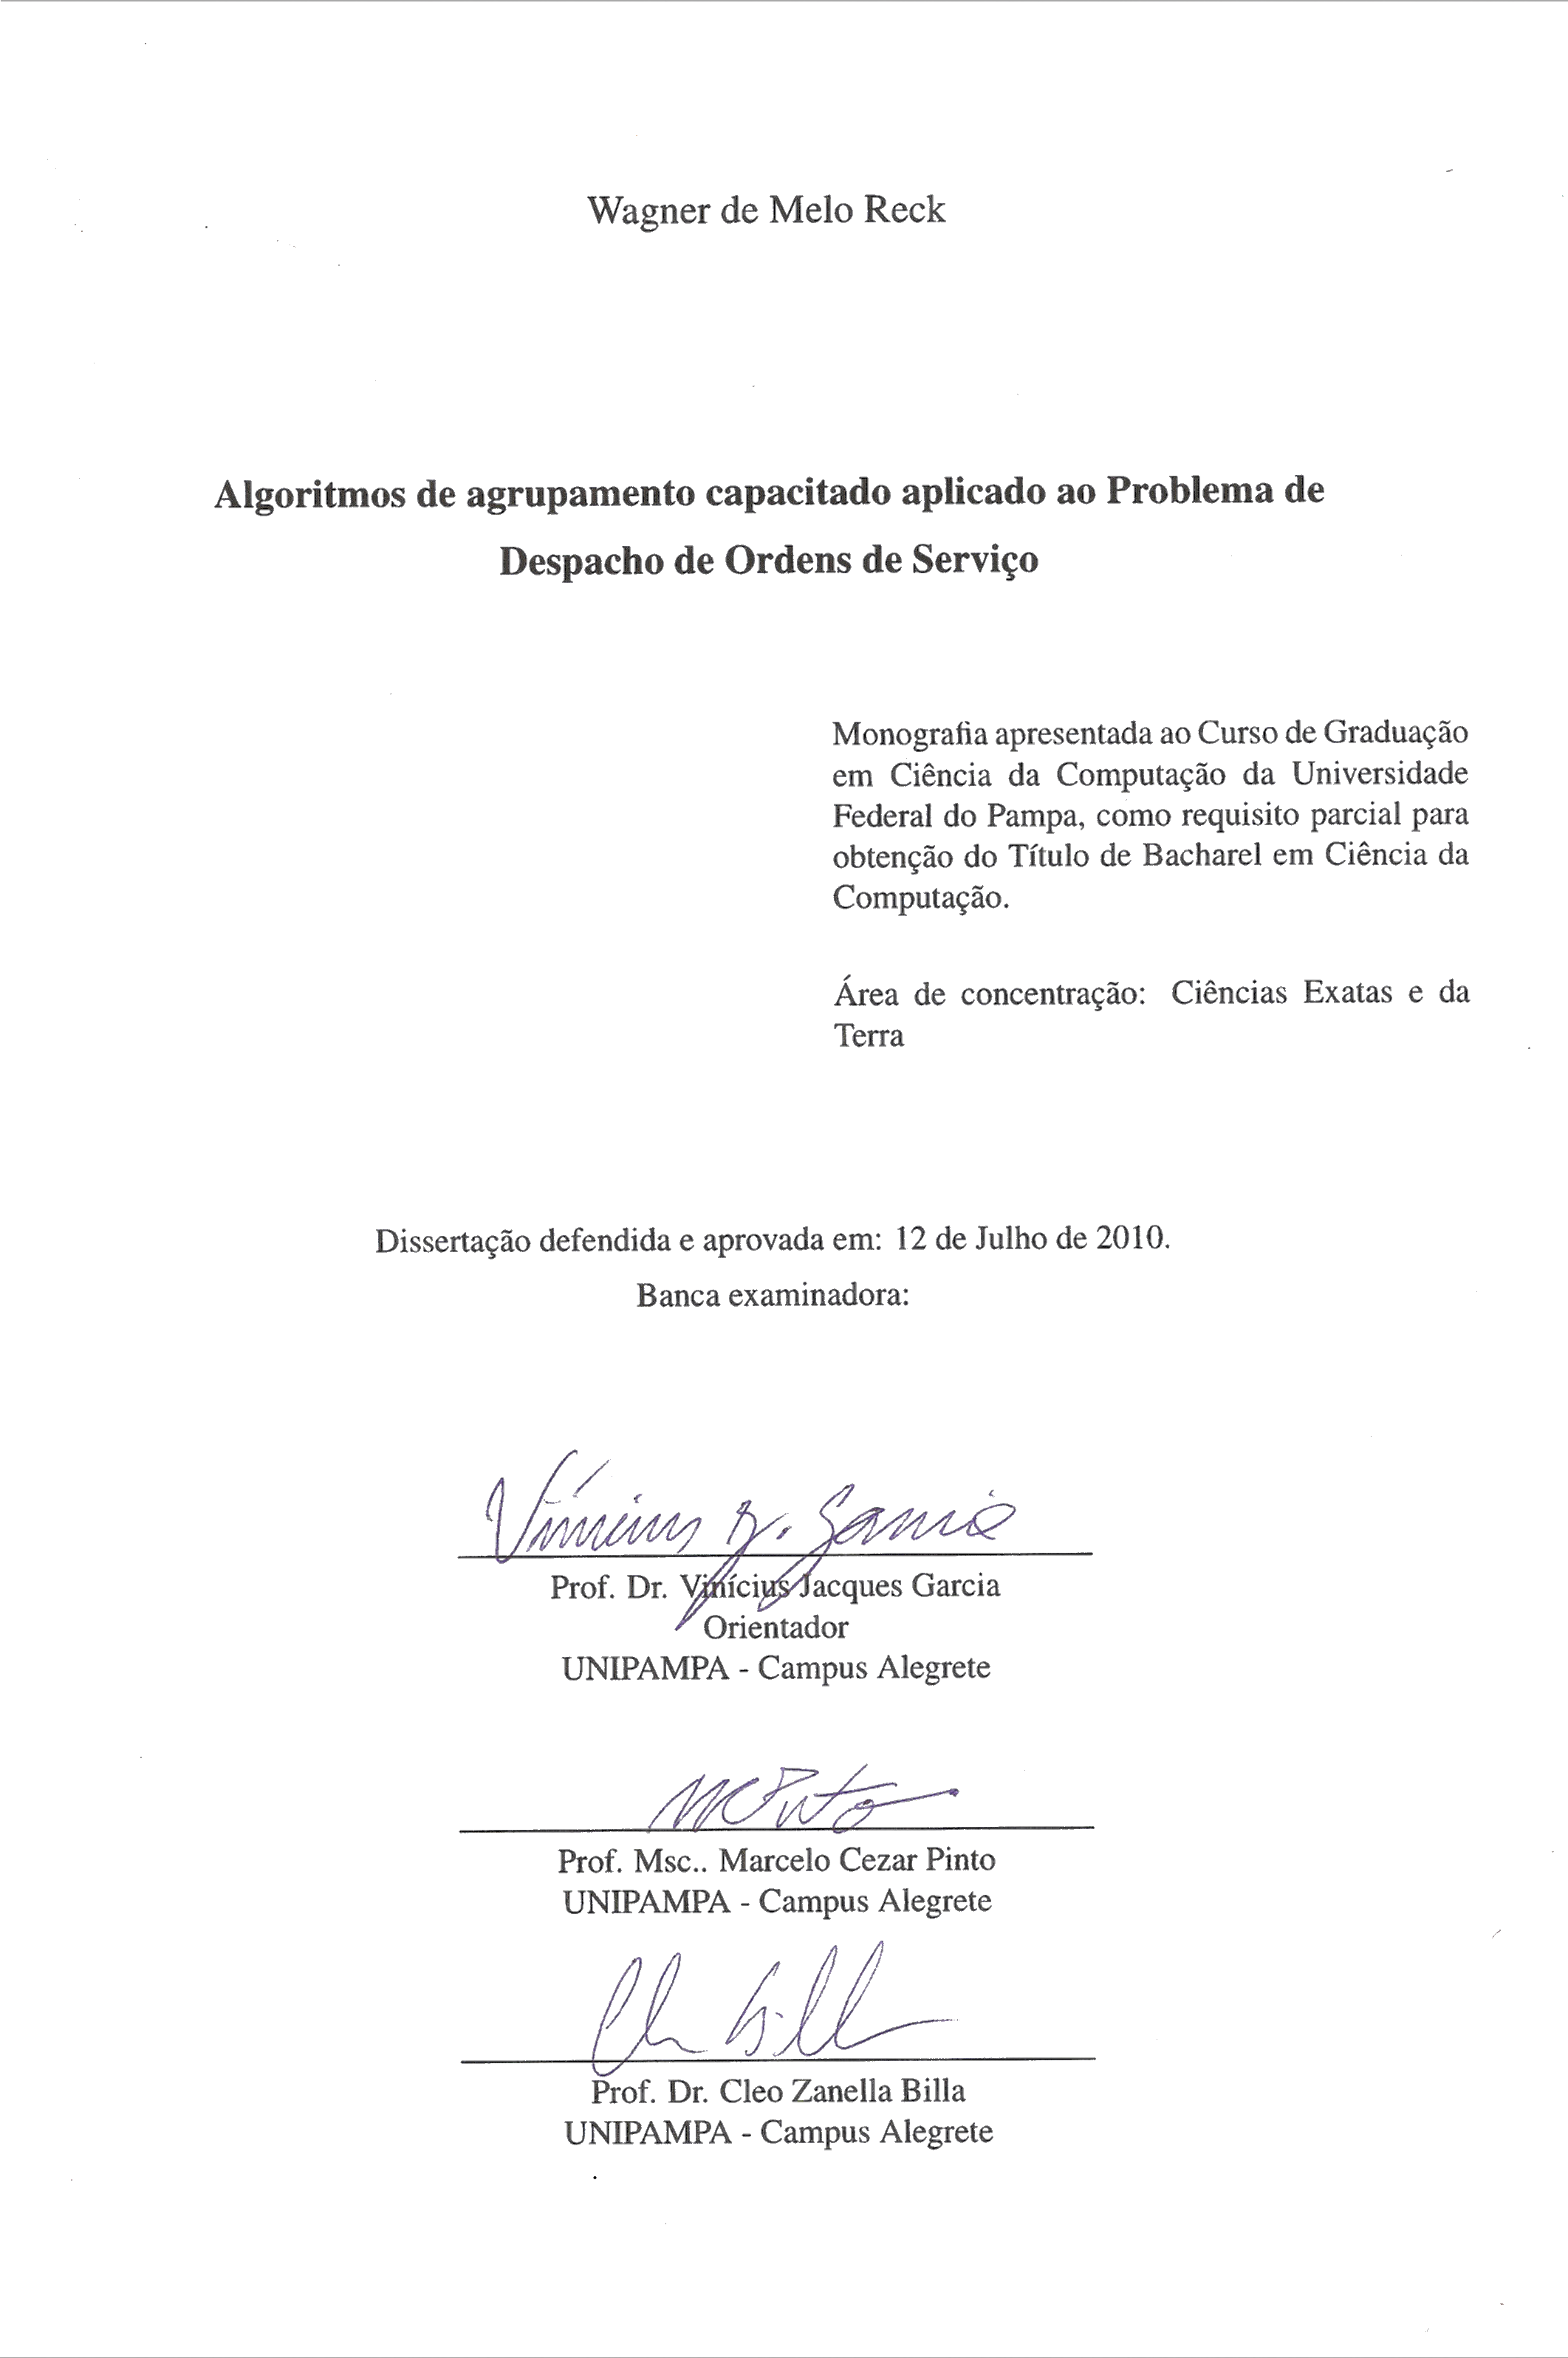
\includegraphics[width=\paperwidth,height=0.9\paperheight,
% keepaspectratio]{./images/ficha_aprovacao.png}%
% % \restoregeometry{}
% %  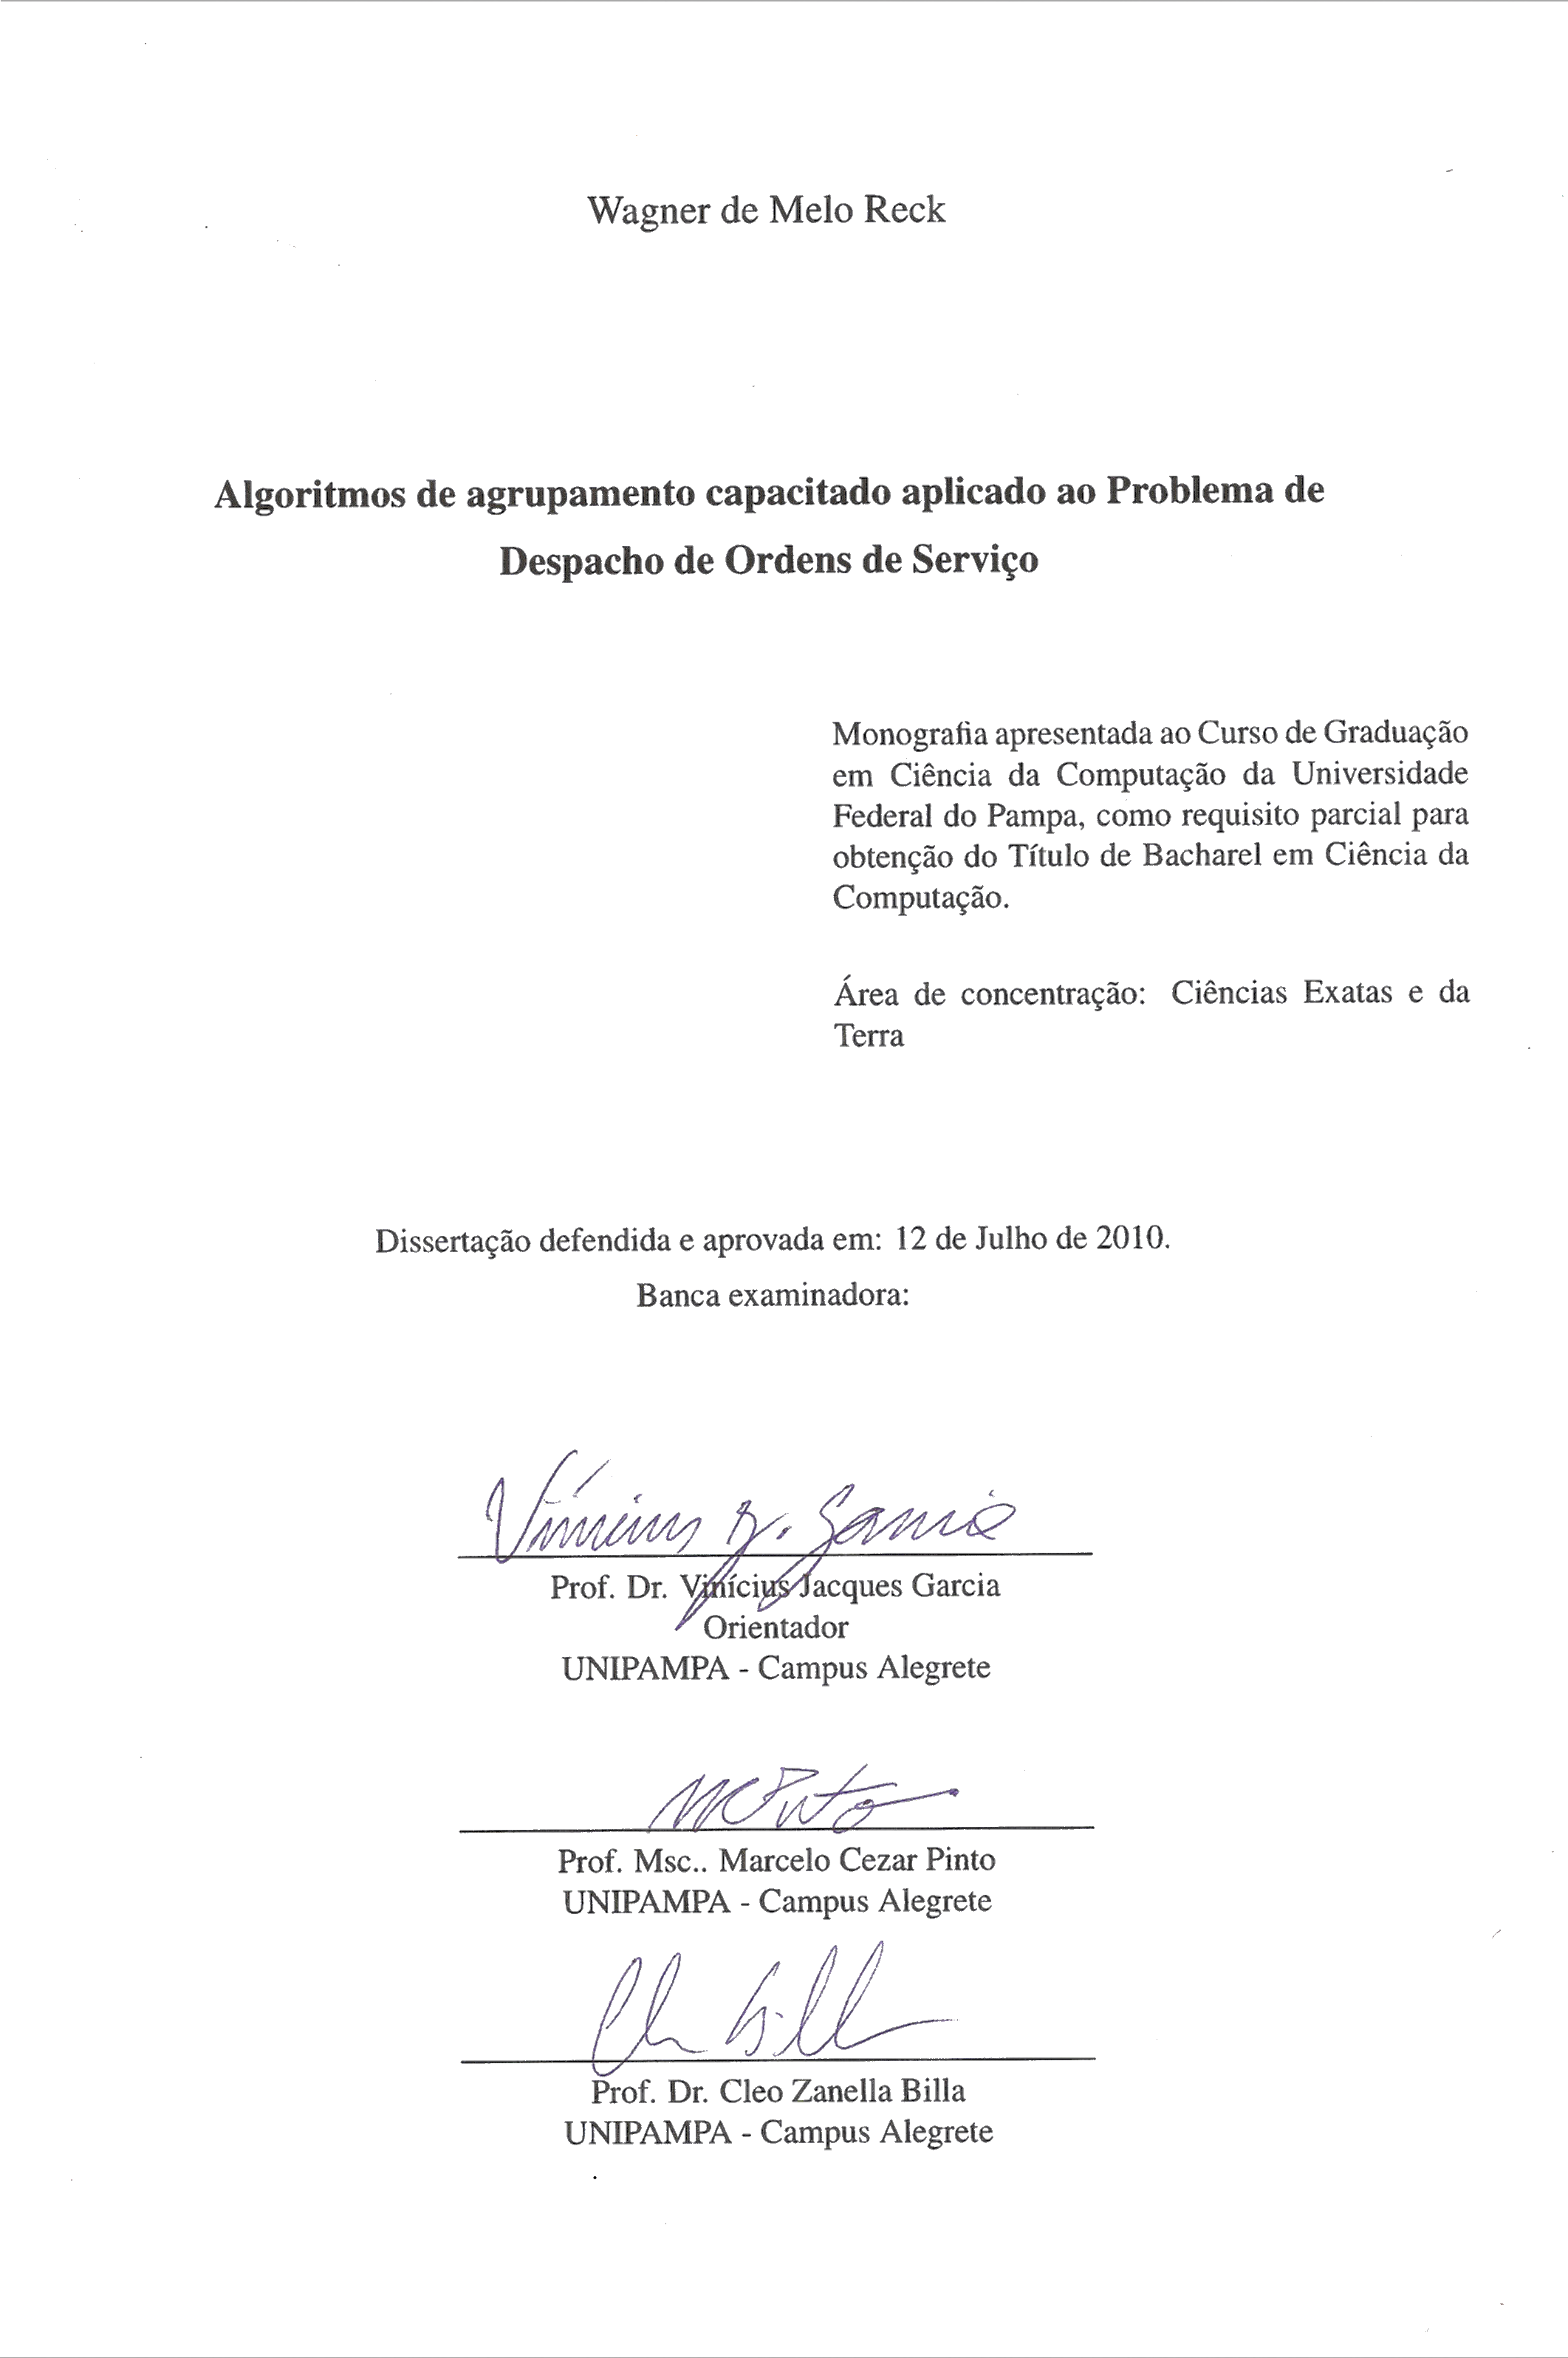
\includegraphics[scale=0.32]{./images/ficha_aprovacao.png}
% %  % ficha_aprovacao.png: 2123x3192 pixel, 96dpi, 56.16x84.44 cm, bb=0 0 1592 2394
% \end{center}
% \end{titlepage}

% \put(0,0){
% \parbox[b][\paperheight]{\paperwidth}{%
% \vfill
% \centering
% 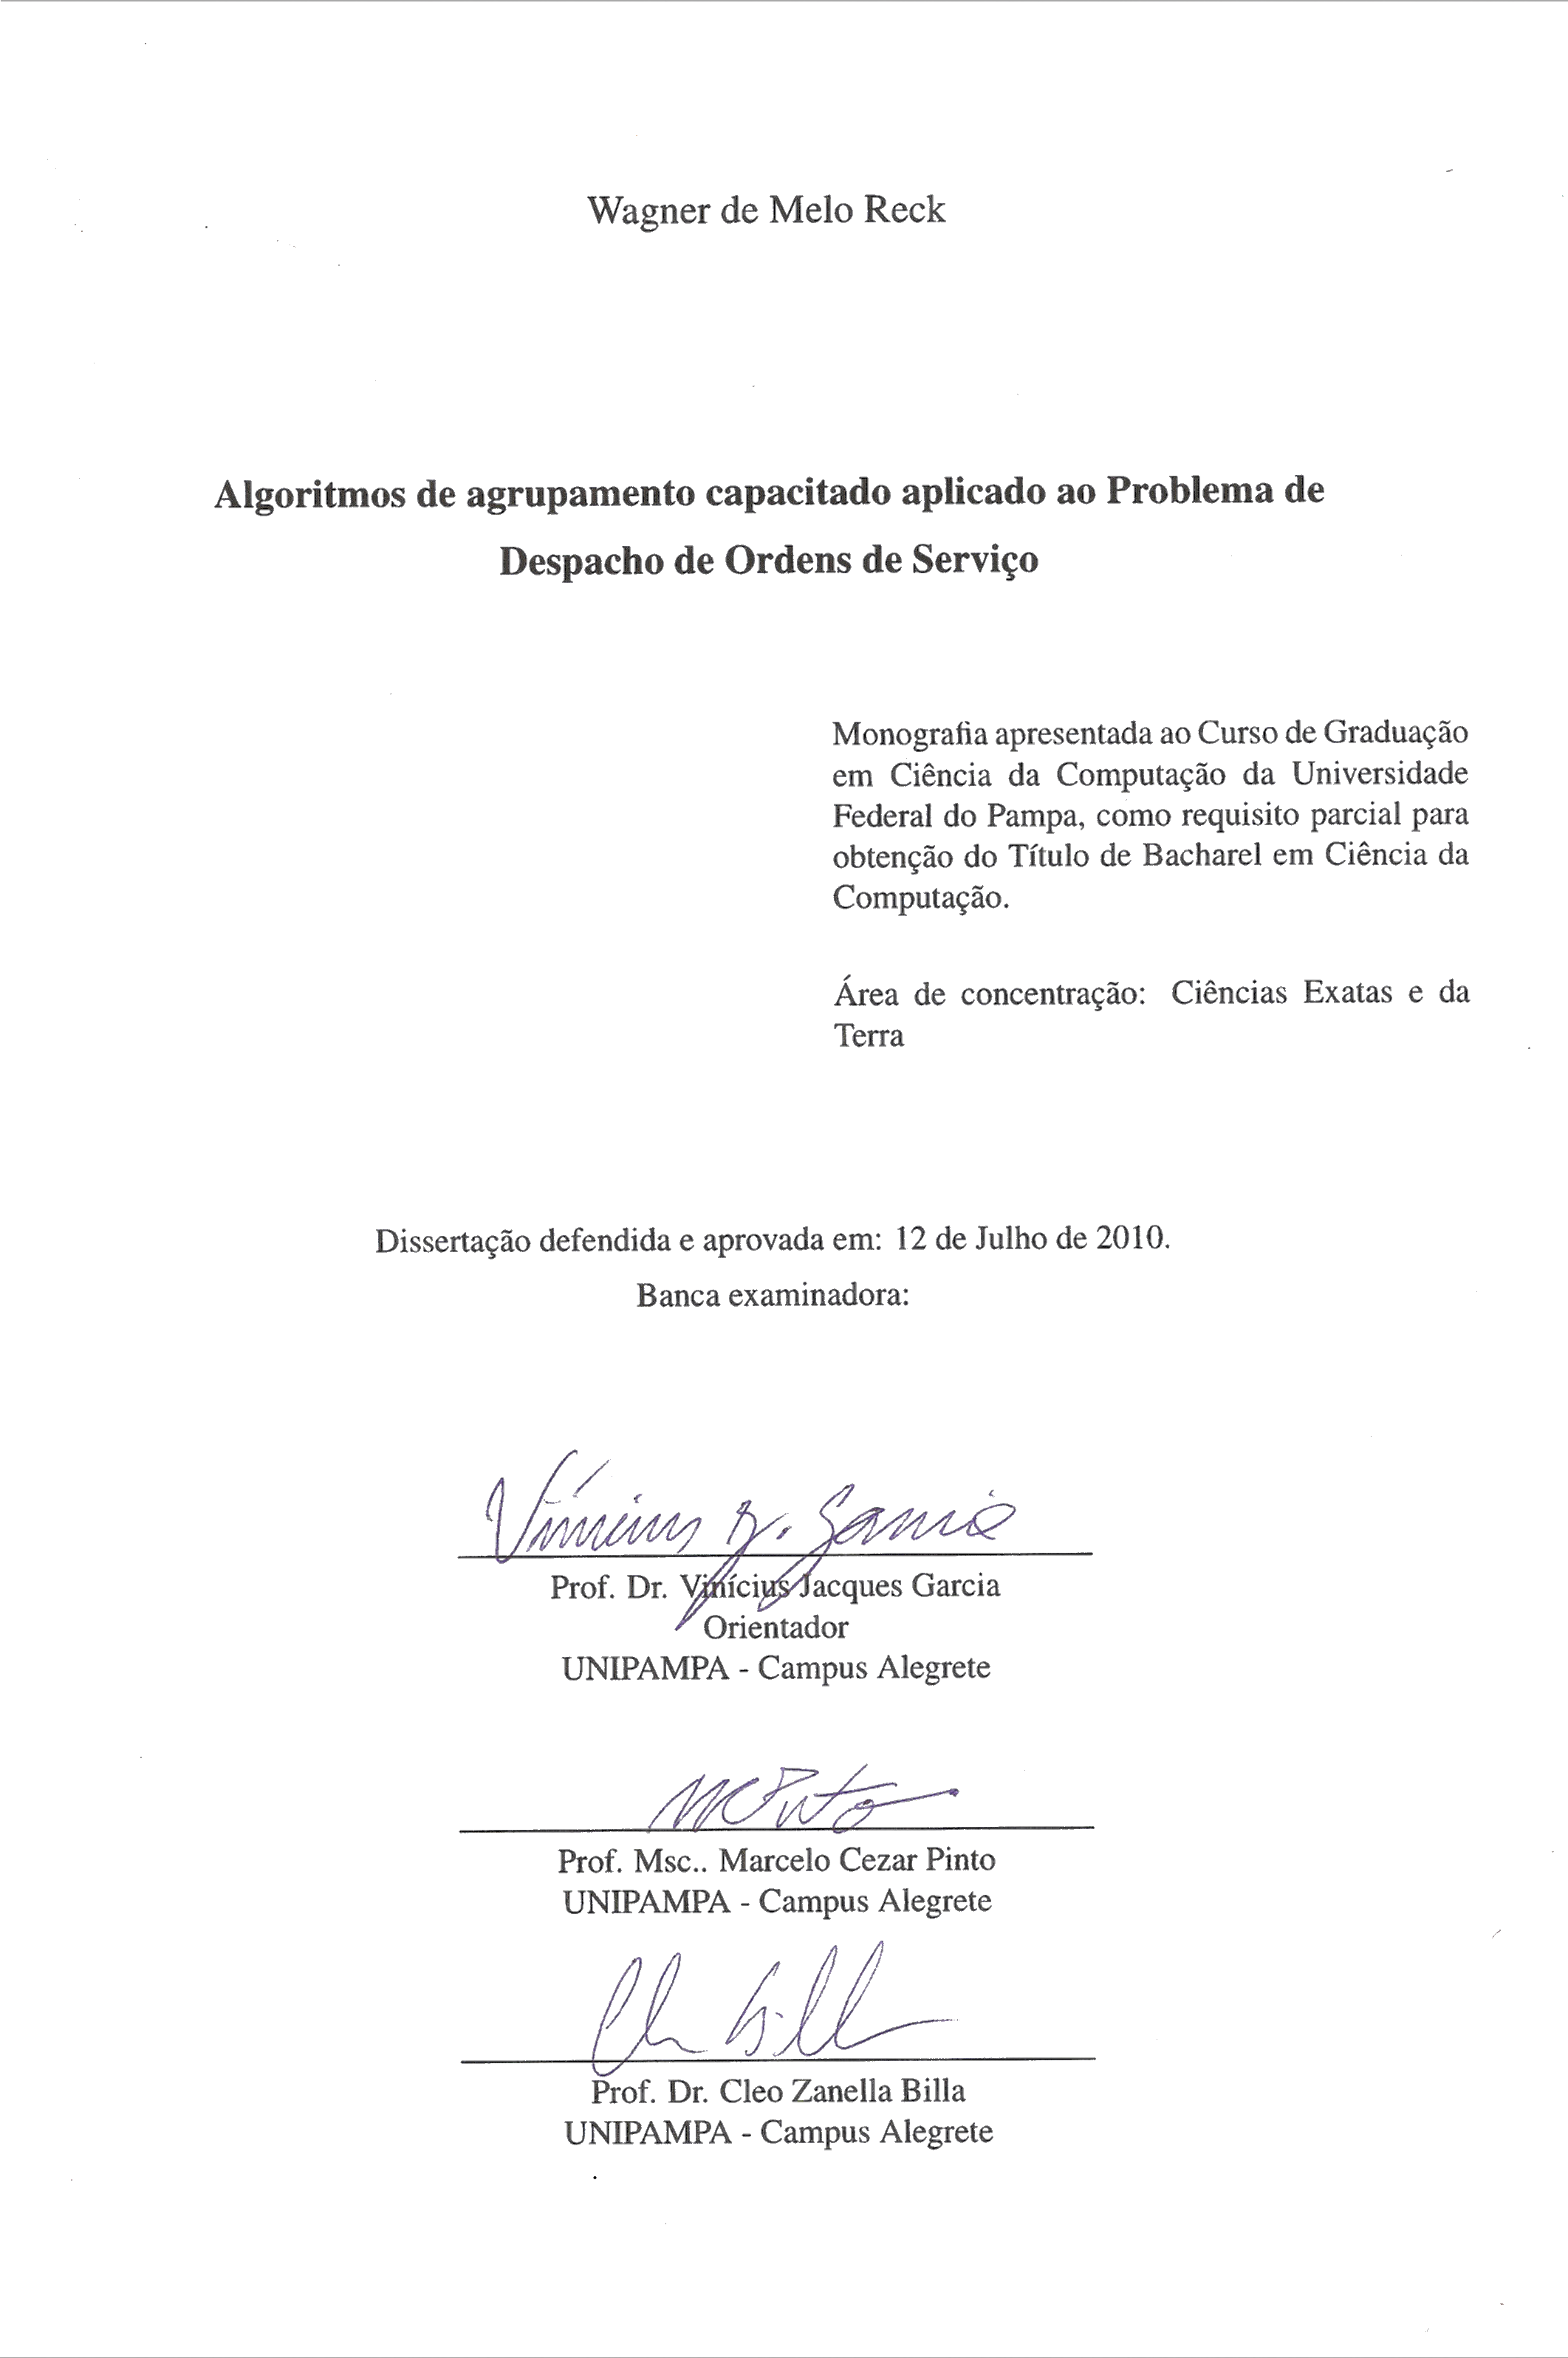
\includegraphics[width=\paperwidth,height=\paperheight,
% keepaspectratio]{./images/ficha_aprovacao.png}%
% \vfill
% }
% }

\vspace{0.75cm}

\begin{center}
	\large\ABNTautordata
\end{center}

\vspace{1.5cm}

\begin{center}
	\large\ABNTtitulodata
\end{center}

\vspace{1cm}

\hspace{8cm}
\begin{minipage}{8cm}
\begin{espacosimples}
Exame de qualifica��o apresentada ao Programa de P�s-gradua��o \textit{Strictu Sensu} em
Engenharia El�trica da Universidade
Federal do Pampa, como requisito
parcial para obten��o do T�tulo de
Mestre em Engenharia El�trica.
\vspace {0.7cm}
\\�rea de concentra��o: Ci�ncias Exatas e da Terra

\end{espacosimples}
\end{minipage}

\vspace {1cm}
\begin{center}
Exame de qualifica��o defendido e aprovada em: 6 de Janeiro de 2012.\\
Banca examinadora:
\end{center}
\vfill

\setlength{\ABNTsignthickness}{0.4pt}
\setlength{\ABNTsignskip}{2cm}

\vspace{-0.5cm}
\assinatura{Prof. Dr. Vin�cius Jacques Garcia\\Orientador\\UNIPAMPA - Campus Alegrete}

\vspace{-0.5cm}
\assinatura{Prof. Dr. Daniel Pinheiro Bernardon\\UNIPAMPA - Campus Alegrete}

\vspace{-0.5cm}
\assinatura{Prof. Dr. Mauricio Sperandio\\ UNIPAMPA - Campus Alegrete}


\end{titlepage}
% Dedicat�ria(s)
% Agradecimentos
% Ep�grafe
% \pretextualchapter{~}

\vfill
\hspace{.3\textwidth}
\begin{minipage}{.6\textwidth}
	\par $\phantom{linha em branco}$
 \begin{flushright}
    \par Dedico esse trabalho � minha amada esposa Joseane, pela paci�ncia, carinho e apoio incondicional em todos meus projetos acad�micos e pessoais.
  \end{flushright}
  \par $\phantom{linha em branco}$
 \end{minipage}

\newpage

% ******** AGRADECIMENTOS *********
% *********** OPCIONAL ************
\pretextualchapter{\textnormal{\textbf{\large{AGRADECIMENTO}}}}

\hspace{.3\textwidth}
	\par Meu primeiro agradecimento vai para minha fam�lia, sem a qual eu n�o estaria aqui vivo. Agrade�o pela paci�ncia e pela compreens�o no momentos que mais precisei (principalmente nos v�rios meses sem visit�-los), pelas palavras de apoio e conforto (\emph{``logo logo termina!''}) e claro pela sua �ndole exemplar e conhecimento �nico que pude desfrutar durante minha vida. Muito obrigado por tudo, pai, m�e e mano, os aplausos s�o para voc�s tamb�m!
    \par Acho que eu n�o estaria aqui, escrevendo esse trabalho, se n�o fosse por meu querido mestre, tutor e amigo, meu professor Vin�cius Jacques Garcia, ao qual eu deve grande parte de meu conhecimento, n�o s� acad�mico mas conduta. Obrigado pelas conversas amigas e paci�ncia com minha d�vidas. Espero trilhar novos caminhos ao teu lado.
    \par Tamb�m deve dizer que sem uma outra pessoa eu n�o estaria aqui, quer dizer, eu at� estaria mas possivelmente tomando algum tarja preta ou em uma consulta num psiquiatra, o que eu quero dizer � que se eu mantenho ainda um pouco de lucidez mental � gra�as a minha amada esposa Joseane (mas chamem-na de J�). Muito obrigado pelos �timos momentos ao seu lado, por ser minha companheira nas minhas id�ias geniais (leia-se loucas), pela for�a nas aulas de c�lculo e por rir das minhas piadas (pelo menos das boas).
    \par Agrade�o ao meu gato, que tem o nome de POG mas ningu�m chama ele por esse nome, por me fazer rir quando tentava pegar o cursor do mouse :).
    \par Tenho um agradecimento especial aos demais professores que me acompanharam e incentivaram durante a gradua��o, compartilhando seu tempo, paci�ncia e conhecimento, contribuindo na minha forma��o. Obrigado Amanda, Vanessa, Diego, MC(Marcelo), Alessandro, Divane, Fabiane, Fernando, Daniel, Rog�rio, Ant�nio, Vin�cius(Montagner), Deise, Eduardo, Cleo.
    \par Al�m do conhecimento na gradua��o levo tamb�m a amizade e companheirismo de v�rios colegas do nosso curso e de outros tamb�m. Obrigado pelos momentos divertidos durante os trabalhos e momentos de estudo. Obrigado Parizi, Rodrigo, Tati, �ngela, Igor, Daniel, Peuchibo e outros tantos que encheriam muitas outras p�ginas.
    \par \#finalDoTCC



% *********** EP�GRAFE ************
% *********** OPCIONAL ************
\pretextualchapter{~}

\vfill
\hspace{.2\textwidth}
\begin{minipage}{.8\textwidth}
	\par \emph{Voc� acha que o seu problema � s�rio? | exclamou Marvin, como se estivesse se dirigindo ao novo morador de uma sepultura | E eu? O que eu fa�o se eu sou um rob� man�aco-depressivo? N�o, nem tente me responder; eu sou 50 mil vezes mais inteligente que voc� e nem eu sei a resposta. S� de tentar me colocar no seu n�vel intelectual, fico com dor de cabe�a.}
	\begin{flushright}
\par Douglas Adams | O Guia do Mochileiro das Galaxias                                                        \end{flushright}
\end{minipage}

% Resumo em l�ngua vern�cula - Obrg
\begin{resumo}
$\phantom{linha em branco}$\\
\noindent Falar que o sistema ser� colocado em opera��o na AES? n�o falar sobre a ASE em si, mas que pode ser usado em concession�rias

\noindent Este\\

$\phantom{linha em branco}$\\
\begin{espacosimples}
Palavras-chave: PO; Heur�sticas; PAC, Agrupamento.
\end{espacosimples}
\end{resumo}

% *********** ABSTRACT ************
\begin{abstract}
$\phantom{linha em branco}$\\
\noindent With.

\noindent This.\\
$\phantom{linha em branco}$\\

\begin{espacosimples}
Key-words: OR; Heuristic; CCP, Clustering;
\end{espacosimples}
\end{abstract}
% Resumo em l�ngua estrangeira - Obrg
% Lista de ilustra��es
\listadefiguras
% Lista de tabelas
\listadetabelas
% Lista de abreviaturas e siglas
\listadesiglas
% Lista de s�mbolos
% Sum�rio - Obrg
\sumario

% ELEMENTOS TEXTUAIS
% Introdu��o Obrg
\chapter{Introdu��o}

% A demanda por uma melhor qualidade no fornecimento de energia el�trica, tanto por parte dos consumidores quanto por �rg�o reguladores , como a ANEEL no Brasil, t�m exigido que as empresas concession�rias de distribui��o de energia el�trica investiam na moderniza��o de suas redes sob sua concess�o.

A maior continuidade do fornecimento de energia el�trica � uma demanda por parte dos consumidores e tamb�m uma exig�ncia por org�o reguladores como a ANEEL no Brail, o qual estipula metas de continuidade para as empresas concession�rias atingirem \cite{prodist2010}.

% A demanda por parte dos consumidores e de �rg�o reguladores, como a ANEEL no Brasil, de uma melhor qualidade no , principalmente por uma maior continuidade no fornecimento de energia el�trica, t�m exigido que as empresas concession�rias de distribui��o de energia el�trica investiam na moderniza��o das redes de distribui��o sob sua concess�o.
% elevados pela diminui��o os �ndices de interrup��o, seja pela redu��o da frequ�ncia ou dura��o dos mesmos. Um menor �ndice de interrup��es de fornecimento significa menos penaliza��es decorrentes dessas interrup��es e tamb�m uma menor quantidade de energia n�o suprida, aumentado sua receita.
As concession�rias tentam manter a continuidade do fornecimento o maior poss�vel, visto que a interrup��o gera transtornos para os consumidores e ela deixa de vender energia, mas nem sempre � poss�vel n�o interrompe-lo.  O fornecimento de energia el�trica de um sistema de transmiss�o deve ser interrompido quando a concession�ria necessita executar manuten��es ou expans�es na rede, ou quando algum defeito permanente ocorre (por exemplo o rompimento de um condutor ou a queda de um poste).

No primeiro caso de interrup��o, a concession�ria conseguem programar previamente a regi�o que ficar� sem fornecimento, restringindo a �rea atingida e escolhendo hor�rios que sejam menos problem�ticos. O segundo caso nem sempre pode ser previsto e evitado, mas pode ter suas consequ�ncias minimizadas, como ser� visto a seguir.



% A elimina��o completa de tais interrup��es � uma tarefa quase imposs�vel. A concession�ria deve efetuar reparos preventivos e de expans�es das redes, a��es essas que algumas vezes necessitam ser executadas com o fornecimento interrompido, al�m de tamb�m existirem as interrup��es n�o programadas, como defeitos provenientes de acidentes de tr�nsito ou interp�ries clim�ticas. No primeiro caso a empresa ainda consegue planejaros trabalhos para atingir menos consumidores ou mesmo escolher hor�rios que tal interrup��o cause o menor impacto. J� o segundo caso, que � o que ser� abordado nesse trabalho, trata de eventos adversos e n�o planejados. %os quais s�o quase sempre invevit�veis.

% EXPLICAR MELHOR SOBRE AS FALHAS


Com a preocupa��o permanente de manter os ind�ces de continuidade altos, novos equipamentos e t�cnicas s�o empregados nas redes de distribui��o para que o impacto de tais interrup��es n�o planejadas seja minimizados.

% Isso �  trazendo vantagens para os usu�rios das redes quanto para as empresas concession�rias.
Um exemplo largamente utilizado � o uso de equipamentos de prote��o e sua instala��o de forma coordenada e seletiva, assim um defeito � isolado com uma menor �rea afetada pela interrup��o \cite{Alguem1988}. Essa metodologia, que � largamente utilizada nas redes de distribui��o, consegue isolar a �rea afetada atrav�s da abertura de equipamentos de prote��o como religadores e chaves fus�veis.

A principal caracter�stica dessa metodologia � o fato de que quando acontece um defeito ela apenas isola o defeito e n�o considera que parte dos clientes podem ser restabelecidos transferindo sua carga para alimentadores vizinhos. Essas transfer�ncias devem ent�o ser calculadas por operadores da rede, com base nos dados de localiza��o do defeito enviados por equipes de campo, para ent�o despachar equipes para executas as manobras. Isso demanda que equipes de manuten��o se desloquem at� a prov�vel localiza��o do defeito (equipamento atuado), para ent�o percorrer a rede e encontrar o defeito, e ent�o receber a indica��o do operador das chaves que devem ser operadas, o que demanda o deslocamente at� elas e isso pode demorar devido as dist�ncias entre as chaves. Ap�s isso tudo, as equipes ent�o  executam os procedimentos de manobra para transferir as cargas.

Esse tempo de deslocamento das equipes para operar as chaves pode ser reduzido com o uso de equipamentos telecomandados. Tais equipamentos permitem que o operador possa enviar comandos para as chaves sem a necessidade de deslocar equipes at� as mesmas. Mas ainda reca� para as equipes encontrarem a localiza��o do defeito e para o operador simular novas topologias de redes. Tais simula��es s�o necess�rias para evitar sobrecargas no sistema, o que poderia levar a novas falhas na rede.

Com o poder computacional cada vez maior e a evolu��o dos sistemas que rodam sobre tais sistemas, juntamente com a crescente disponibilidade de tecnologias de comunica��o remota como as redes de celular e internet, � poss�vel utilizar tais sistemas para prover intelig�ncia computacional para simula��es e enviar os resultados para equipamentos distantes v�rios quilometros uns dos outros. � imagin�vel que com essas tecnologias se possa automatizar a opera��o de redes de distribui��o \cite{somebody}. As redes que utilizam dessas potencialidades, e apresentam algumas caracteristicas que ser�o apresentadas mais a frente nesse trabalho, s�o chamadas redes inteligentes (smarts grids)\cite{MaisAlgu�m} << Ver sobre smart grids
% Para agilizar esse processo, e tamb�m reduzir o n�mero de consumidores com o fornecimento de energia el�trica interrompido, foi desenvolvida uma metodologia para restabelecimento autom�tico em caso de conting�ncia na rede que utiliza os equipamentos telecomandados.


\section{Objetivos}

A metodologia desenvolvida objetiva restabelecer o fornecimento de energia el�trica para, ap�s a ocorr�ncia de um defeito permanente, o m�ximo de consumidores de uma rede de distribui��o, isso de maneira autom�tica sem a necessidade de interven��o humana ou programa��o pr�via das a��es a serem tomadas. Com essa automatiza��o, a metodologia aqui descrita consegue reduzir o tempo de restaura��o da energia para os clientes n�o atingidos pelo defeito.

Para conseguir isso, essa metodologia � capaz de detectar a localiza��o do defeito, e com essa informa��o definir e enviar os comandos a serem executados pelos equipamentos telecomandados. Ela faz uso de v�rias tecnologias para conseguir essa capacidade, dentre elas est�o o uso de um sistema de controle, supervis�o e aquisi��o \sigla{SCADA}{Sistema de Supervis�o e Aquisi��o de Dados - Supervisory Control and Data Aquisition}(SCADA) e de sistemas computacionais inteligentes para defini��o das manobras a serem executadas e simula��es dessas manobras.

Como informa��es de entrada, al�m da topologia inicial da rede, a metodologia tamb�m necessidade de outros dados de entrada, sendo eles o estado atual da rede, uma vez que a topologia origial pode ser alterada e um hist�rico de carregamento da rede para que se possa realizar estima��es de crescimento de carga. O segundo conjunto de dados � necess�rio para estimar se a carga do sistema ir� crescer num horizonte de algumas horas a frente, o que pode gerar sobrecargas no sistema j� que a rede estar� operando fora de sua topologia otimizada ap�s o restabelecimento.

Resalta-se que essa metodologia foi desenvolvida para ser uma m�todo de restabelecimento universal que pode ser aplicado em redes com diferentes topologias e em tempo real, o que traz uma diminui��o significativa do tempo de restabelecimento dos consumidores.

%a fim de restabelecer o m�ximo de consumidores n�o afetados pelo defeito.

% Como isso � feito? � seguro? porque � melhor ? qual a base de funcionamento (sinaliza��o de chaves, eventos de desarme)

\section{Organiza��o desse Trabalho}

Este trabalho est� organizado da seguinte forma:

No Cap�tulo 2 � feito uma revis�o do estado da arte sobre o problema de restabelecimento de redes, automa��o de redes, redes inteligentes e sobre reconfigura��o automatizada.

No Cap�tulo 3 � apresentada uma abordagem ao funcionamento dos sistemas de pot�ncia, com grande enfoque nos sistemas de distribui��o. Tamb�m � abordado a quest�o de automa��o das redes de distribui��o e como � executado o restabelecimento do fornecimento em tais redes. S�o apresentadas m�tricas de medida de desempenho da rede em rela��o a continuidade. Ao final � feita uma compara��o entre a metodologia tradicional de restabelecimento e o m�todo automatizado.

A metodologia � explicada no cap�tulo 4. Ela � dividida em se��es para facilitar o seu entendimento. Inicialmente � feita uma revis�o do problema e quais s�o as fun��es objetivo bem como as restri��es que devem ser consideradas. Em seguida � apresentada a arquitetura imaginada para obten��o de informa��es em tempo real, o que � vital para um melhor resultado da metodologia, e tamb�m � apresentado, sem entrar em detalhes de implementa��o, como se d� essa comunica��o. A descri��o dos algoritmos de tomada de decis�o, o qual enumera as possibilidades de manobras e escolhe dentre elas a melhor a ser executada, � apresentado na sec��o \ref{sec:AlgoritmoTomadaDecisao}.

Os resultados, bem como a descri��o dos ambientes de teste e os dados de entrada, est�o apresentados no cap�tulo \ref{cap:casosestudos}. Nele � apresentado como a metodologia foi testada e implementada em um ferramenta computacional, para depois apresentar alguns testes de restabelecimento em redes e uma an�lise sobre tais resultados.

No cap�tulo \ref{cap:consideracoesFinais} s�o apresentadas as considera��es finais desse trabalho bem como id�ias de trabalhos futuros que podem ser derivados deste trabalho.


 %Inclui arquivo introducao.tex
% % Desenvolvimento - Obrg
\chapter{Revis�o Bibliogr�fica}

Esse cap�tulo traz uma revis�o dos temas de automa��o e restabelecimento, com foco no restabelecimento automatizado, das redes el�tricas. Tamb�m � apresentado alguns conceitos de redes inteligentes (smart grids) e onde este trabalho se encaixa nesse conceito.


O termo \textit{smart grids} vem sendo utilizado para designar as redes do futuro, as chamadas redes inteligentes. Essas redes inteligentes n�o s�o uma tecnologia ou um produto, mas sim um conceito que independe da tecnologia ou dos produtos usados \cite{Falcao2010, Ipakchi2009}. As redes inteligentes s�o assim chamadas por utilizarem a automa��o da rede, sistemas de comunica��o e intelig�ncia computacional para ter um maior controle sobre a rede de distribui��o.
Apesar do termo redes inteligentes tratar desde a gera��o at� as unidades consumidoras, o termo normalmente � aplicado apenas na etapa de distribui��o \cite{Hassan_Radman_2010}.

As redes inteligentes normalmente t�m as seguintes caracter�stica a elas atribu�das \cite{Falcao2010}:
\begin{itemize}
 \item Toler�ncia a ataques externos, seja eles cibern�ticos ou f�sicos;
 \item Maior qualidade de energia para os consumidores finais;
 \item Participa��o do consumidores como produtor de energia el�trica (micro gera��o);
 \item Capacidade de acomodar uma diversidade de fontes geradoras de forma transparente;
 \item Reduzir as perdas e com isso diminuir o impacto ambiental;
 \item Auto recupera��o: Capacidade da rede restabelecer-se ap�s a ocorr�ncia de um defeito de forma aut�noma.
\end{itemize}

\textbf{Quais s�o as caracter�sticas das redes inteligentes? Falar de redes automatizadas e aut�nomas. Redes capazes de se auto-recompor (self healing). Medi��es em tempo real. Reconfigura��o autom�tica }

Esse � um tema que est� sendo tratado atualmente em diversos trabalhos \cite{Ipakchi2009,Farhangi2010,Moslehi2010}, uma vez que est�o sendo definidas as tecnologias que implementam o que era definido apenas como conceito. As redes inteligentes necessitaram de uma intelig�ncia computacional para que sejam capazes de tratar de diferentes situa��es que acontecem no dia-�-dia de uma rede de distribui��o. Um trabalho nessa �rea � o estudo do uso de agentes inteligentes para gerenciar tais redes\cite{filipe2012aplicacao, Falcao2010, Soo2010}. Apesar de essa ser uma forma de representar, existem outros trabalhos que n�o fazem uso desse tipo de intelig�ncia artificial, mas fazem uso de heur�sticas e bases de conhecimento\cite{Teo1992,curcic1996electric, maisAlgum}.

Essas chamadas redes inteligentes fazem uso de diferentes tecnologias, de informa��o, comunica��o e automa��o, o que aumenta a sua complexidade \cite{Moslehi2010}. As diferentes tecnologia utilizadas nessas redes est�o em constante evolu��o, seja pelo desenvolvimento de novos equipamentos ou pela defini��o de padr�es de projeto para uso em tais redes \cite{Singhal2012}.

\textbf{Ressaltam-se tamb�m as primeiras experi�ncias pr�ticas sobre o uso dessas redes inteligentes, como a cidade de �vora em Portugal.} \textbf{Procurar por outras experi�ncias pr�ticas}



%%%%%%%%%%%%%%%%%%%%%%%%%%%%%

Reconfigura��o das redes trata sobre a altera��o da topologia da rede atrav�s da abertura e fechamento de chaves, sendo a maioria dos estudos sobre a melhoria da qualidade de energia e redu��o das perdas \cite{Braz2011,Radha2010,Souza2010}. A reconfigura��o da rede tamb�m � tratado quando desejamos restaurar a rede em situa��es de falhas, ap�s a mesma ter apresentado algum defeito e desejamos restabelecer o m�ximo de consumidores, deixando apenas a �rea afetada pelo defeito desenergizada\cite{Garcia2005}. Esse tipo de reconfigura��o tamb�m � referenciado como restabelecimento.

O estudo da reconfigura��o da rede � tido como sendo de natureza combinat�ria \cite{Souza2010}, n�o sendo poss�vel, em casos reais, testar todas as possibilidades devido ao alto custo computacional envolvido. Para resolver o problema de reconfigura��o, normalmente s�o aplicadas heur�sticas para encontrar a melhor solu��o poss�vel em um espa�o de tempo aceit�vel.

Levando em considera��o a import�ncia da solu��o r�pida e eficiente do restabelecimento do fornecimento de energia em situa��es de conting�ncia, tanto para as concession�rias quanto para os consumidores, este assunto � discutido em um grande n�mero de publica��es realizadas durante um longo per�odo de tempo \cite{castro1980, Kuwabara1987, Ucak1994, nagata2001efficient}. Primeiramente, estas pesquisas foram direcionadas somente para a an�lise dos sistemas de pot�ncia \cite{teo1992computer, kojima1989development}. Nos anos noventa, surgiram situa��es em que a confiabilidade dos sistemas de pot�ncia tornou-se muito maior que a dos sistemas de distribui��o. Os dados apresentados em v�rios pa�ses mostraram que as falhas nos sistemas de distribui��o eram respons�veis por cerca de 90\% do tempo em que os consumidores ficavam sem fornecimento.

\textbf{Nesse cen�rio cada vez mais s�o desenvolvidas pesquisas voltadas para o aumento da confiabilidade dos sistemas de distribui��o\cite{aoki1989new, lin1998new, zhou1997distribution}, e mais recentemente no que se refere as redes inteligentes \cite{Moslehi2010,Adhikari2009,Soo2010,Podmore2010a}.
Por isto, no processo de implanta��o dos equipamentos de inform�tica, desenvolvimento de sistemas de controle e instala��o nas redes de equipamentos de comuta��o telecomandados, cresce a quantidade de pesquisas voltadas para o aumento da confiabilidade dos sistemas de distribui��o, em particular as ligadas com o desenvolvimento de m�todos de restabelecimento �timo do fornecimento de energia em situa��es de conting�ncia \cite{Adhikari2009,Soo2010,Podmore2010a} %.
A aten��o principal dos pesquisadores est� voltada para a busca de m�todos eficientes de otimiza��o, levando em conta a extrema complexidade deste problema combinatorial de grandes dimens�es.}

Eram claramente conhecidas as dificuldades ligadas com a tentativa de utiliza��o de m�todos cl�ssicos de programa��o matem�tica para a solu��o deste problema \cite{curcic1996electric}. Por isto, os esfor�os dos pesquisadores foram direcionados para a an�lise da possibilidade de utiliza��o de v�rios m�todos heur�sticos de otimiza��o \cite {moon2000fault}, por exemplo, redes neurais \cite{bretas2001fault}, redes Petri \cite{fountas1997hierarchical, wu1998petri} ou mesmo sistemas especialistas baseados em regras \cite{Ma1992}.

Obviamente, a eficiente solu��o daquele problema era
imposs�vel sem a utiliza��o do conhecimento e experi�ncia da equipe dos setores de opera��o das concession�rias. Primeiramente, isto foi realizado a partir do desenvolvimento de sistemas especialistas \cite {liu1988expert, Ma1992, wu1997enhancement, nagata1995power}. A desvantagem destes trabalhos � que a grande maioria praticamente ignora a totalidade da informa��o formal que est� dispon�vel nas concession�rias. Por esta raz�o, torna-se mais eficiente considerar algoritmos que possibilitem reunir m�todos de an�lise formais e heur�sticos. \cite{hsu1991distribution, morelato1989heuristic, drezga2001object}.

Da mesma forma, conforme j� mencionado, o problema de defini��o da configura��o �tima das redes de distribui��o, ap�s as falhas, n�o pode ser solucionado de forma correta e eficiente sem a an�lise de problemas como: modelagem adequada e previs�o de cargas dos transformadores de distribui��o, c�lculos das perdas de energia e n�veis de tens�o, considera��o sobre a prioridade dos consumidores e, a seguir, tomadas de decis�o com base em m�todos de an�lise multicriterial. � necess�rio ressaltar que os trabalhos que analisam este problema sob tal formula��o geral, s�o a minoria \cite{miu1998fast, hsu1994heuristic, popovic1999multi}.

Consequentemente, o desenvolvimento de um m�todo eficiente e universal para a an�lise do problema em quest�o � extremamente dif�cil, levando em conta a grande quantidade de fatores a serem considerados.

\textbf{Assim, conforme as experi�ncias e de acordo com a an�lise bibliogr�fica, pode-se atingir solu��es mais eficientes quando o problema � resolvido para cada concession�ria, individualmente, considerando a estrutura das redes de distribui��o, quantidade e composi��o dos equipamentos de comuta��es, opera��o do sistema SCADA, sufici�ncia e adequa��o da informa��o inicial \cite{nahman1994new, lei2000network, lee1998service}.}


\textbf{Trabalhos com heur�sticas: Falar de alguns outros algoritmos e redes inteligentes}

%%%%%%%%%%%%%%%%%%%%%%%%%%%%%%%%%%%%
Normalmente, esse restabelecimento do fornecimento nas redes � realizado por meio da opera��o manual das chaves, sendo necess�rio que as equipes se desloquem at� as mesmas. Para tornar esse processo mais r�pido, � poss�vel automatizar essa opera��o atrav�s da automa��o dos equipamentos de manobra da rede \cite{ Sperandio2008}.

\textbf{Falar o que � a automa��o da rede. Depois tratar como essa automa��o vem sendo aplicada nas redes de distribui��o. Trabalhos relacionados (ver material do Luciano)}

Tais chaves permitem sua opera��o � dist�ncia sem a necessidade de deslocar equipes.

Essa possibilidade abre espa�o para a automatiza��o das redes\cite{Gris2010}, usando da comunica��o das chaves para obter informa��es de campo e a intelig�ncia computacional para determinar quais chaves devem ser operadas.



\textbf{Desta forma, este trabalho explora parte deste conceito, visto que associa-se as redes inteligentes a caracter�stica de auto-recupera��o das redes, ou seja, a capacidade de automaticamente detectar, analisar, responder e restaurar falhas na rede.
%  \(definir as manobras mais adequadas, verificar a viabilidade t�cnica das mesmas...\)...
%
O diferencial deste trabalho � tratamento combinado das informa��es de campo (monitora��o, controle, aquisi��o de dados...) com simula��es computacionais.}

% No final da revis�o, voc� tem que destacr o seu trabalho, coloca, algo do tipo:
\textbf{Apesar de haver v�rias pesquisas, este tema ainda n�o est� finalizado. Cada vez mais os equipamentos evoluem e s�o capazes de fornecer novas informa��es, as quais podem ser utilizadas em novas metodologias, como por exemplo, para calcular a localiza��o do defeito. Mas para isso � necess�rio o desenvolvimento de m�todos eficientes aplicados para sistemas reais de distribui��o de energia el�trica, com o prop�sito de restabelecimento autom�tico de energia el�trica.}


% \chapter {Sistema de distribui��o de energia el�trica}
% 3 - Sistemas de Distribui��o de Energia El�trica
% 3.1 - Introdu��o � Sistemas de Distribui��o
% 3.2 - Automa��o de Sistemas de Distribui��o
% 3.3 - Procedimento Convencional para Restabelecimento de Energia El�trica

Nesse cap�tulo ser�o descritos os sistemas de distribui��o de energia el�trica em m�dia tens�o, abordando conceitos b�sicos sobre distribui��o que servir�o de base para a apresenta��o da metodologia no decorrer deste trabalho. Al�m dos conceitos sobre o funcionamento de tais sistemas, tamb�m ser� abordado a ocorr�ncia e solu��o de defeitos (situa��es de conting�ncia) bem como a automa��o dos sistemas de distribui��o.

Um sistema el�trico de pot�ncia tem por fun��o prim�ria a entrega de energia el�trica para consumidores finais (casas, industrias,...) sendo composto por uma fonte geradora, que ir� transformar algum tipo de energia, seja ela hidr�ulica, t�rmica ou outra, em energia el�trica a qual ser� distribu�da para os consumidores atrav�s de diferentes redes de transmiss�o/distribui��o at� os consumidores finais\cite{Nelson_Kagan_Introd}. Como n�o � poss�vel de efetuar o armazenamento de tal energia, o sistema deve estar pronto para suportar a demanda imediata de seus consumidores sem sofrer de nenhum tipo de sobrecarga nos equipamentos de transporte de energia (condutores, disjuntores) ou mesmo dos equipamentos de gera��o.

Os sistemas el�tricos de pot�ncia possuem a topologia apresentada na figura \ref{fig:SEP}. Podem ser vistos 3 grandes blocos: um de gera��o, um de transmiss�o e outro de distribui��o. Estes blocos maiores tamb�m podem ser subdivididos em outros blocos, como a distribui��o pode ser dividida em sub-transmiss�o e distribui��o prim�ria e secund�ria. O acoplamento entre esses diferentes blocos � dados atrav�s de esta��es elevadoras ou rebaixadoras de tens�o.
\begin{figure}
\begin{centering}
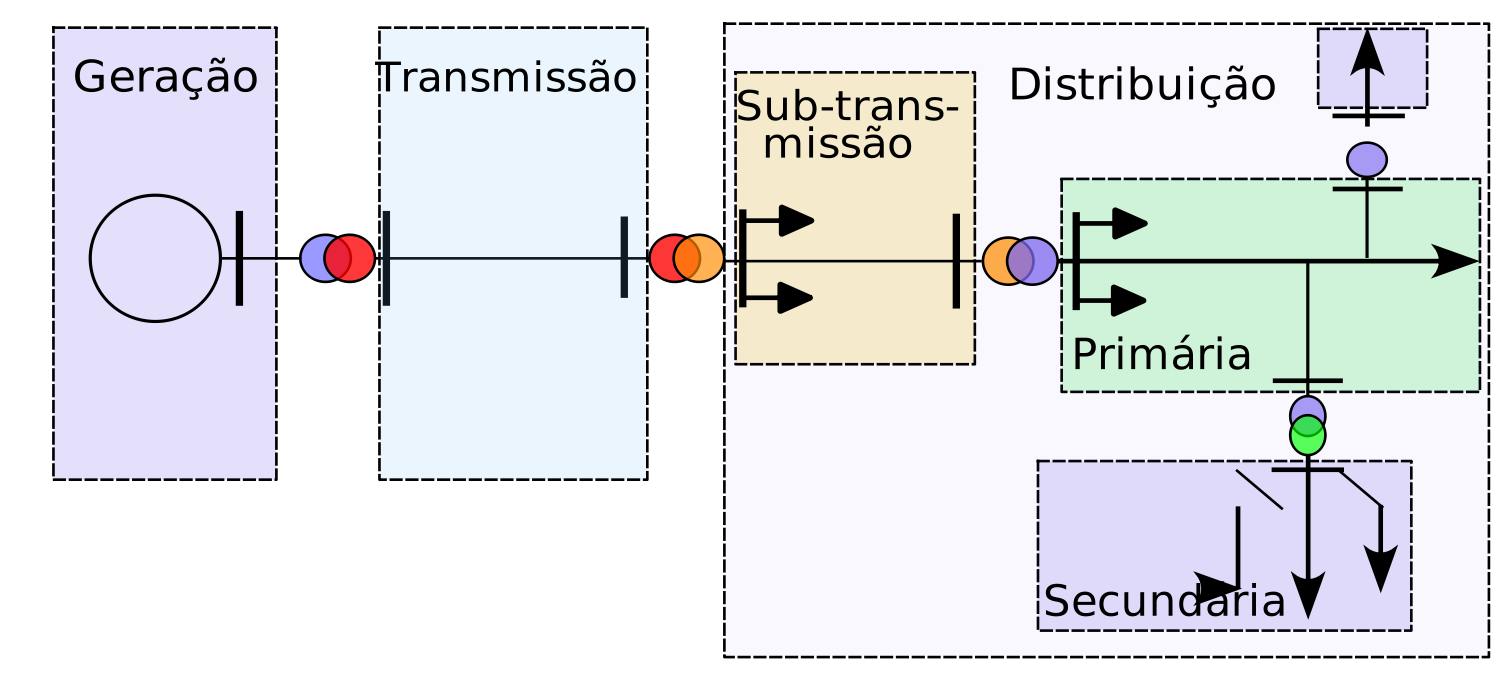
\includegraphics[width=0.8\columnwidth]{img/SEP}
\par\end{centering}

\caption{Exemplo de Sistema El�trico de Pot�ncia \label {fig:SEP}}
\end{figure}

A etapa de gera��o trata da transforma��o de alguma energia em energia el�trica, como por exemplo uma hidroel�trica que faz uso de alguma queda d'�gua para fazer as turbinas girarem que por sua vez s�o acopladas a conjuntos geradores como alternadores. Existem tamb�m outras formas de gera��o de energia como por fiss�o nuclear, queima de combust�veis como madeira, baga�o de cana, �leo combust�vel entre outros, tem nesses casos o objetivo de aquecer a �gua de modo a produzir vapor que faz as turbinas girarem.

Com a energia el�trica gerada, ela deve ser levada at� os consumidores. Uma vez que as grandes centrais geradora se encontram afastadas dos principais centros consumidores, � necess�rio um sistema que transporte a energia por longas dist�ncias e tenha uma baixa perda de energia. Para isso a energia gerada � elevada para a casa de centenas de milhares de volts e s� ent�o � transmitida por longas dist�ncias.

O �ltimo bloco, a distribui��o trata de obter a energia do bloco de transmiss�o e entregar para o consumidor final em tens�es apropriadas conforme a necessidade de cada um. A pr�xima sec��o tratar� sobre esse tema de modo mais abrangente.


\section{Introdu��o � Sistemas de Distribui��o}

Os sistemas de distribui��o de energia el�trica tratam sobre como a energia, depois de ter sido transmitida de um esta��o geradora, � entregue para os consumidores. Para isso o sistema pode ser dividido em sub-transmiss�o, que trata da distribui��o para as subesta��es e consumidores de grande porte, e em dois tipos de distribui��o propriamente dita, uma prim�ria e outra secund�ria, que tratam de como a energia � distribu�da de forma segura e eficiente para a grande parte dos consumidores (resid�ncias e pequenas/m�dias industrias).

A distribui��o prim�ria tem dois componentes importantes as subesta��es e as redes de distribui��o prim�ria, tamb�m conhecidas como alimentadores. As primeiras tem o papel de rebaixar a tens�o recebida da sub-transmiss�o e de proteg�-la contra defeitos de curto circuito. J� as redes de distribui��o prim�ria s�o deriva��es da subesta��o, ou seja, podem existir mais de uma rede de distribui��o em uma subesta��o, e tais redes tem por objetivo entregar energia el�trica diretamente para os consumidores de m�dio porte, como industrias e universidades, como tamb�m para os transformadores que rebaixar�o a tens�o para n�veis residenciais para ser distribu�da pelas rede de tens�o secund�ria.


Uma representa��o de uma rede de distribui��o prim�ria, juntamente com os seus principais componentes, pode ser vista na Fig. \ref{fig:redeDistribui��o}. Cada alimentador tem inicio na subesta��o e possui um equipamentos de prote��o, chamado de disjuntor. Localizado logo ap�s a sa�da da subesta��o, ele respons�vel por impedir que defeitos que apare�am da rede, como postes ca�dos ou contato entre condutores que geram um curto circuito, se propaguem para dentro da subesta��o, o que poderia afetar os sistemas de transmiss�o ou mesmo de gera��o, al�m de impedir que defeitos ocorridos em um alimentar afetem os consumidores que s�o atendidos por outros alimentadores.

\begin{figure}
\begin{centering}
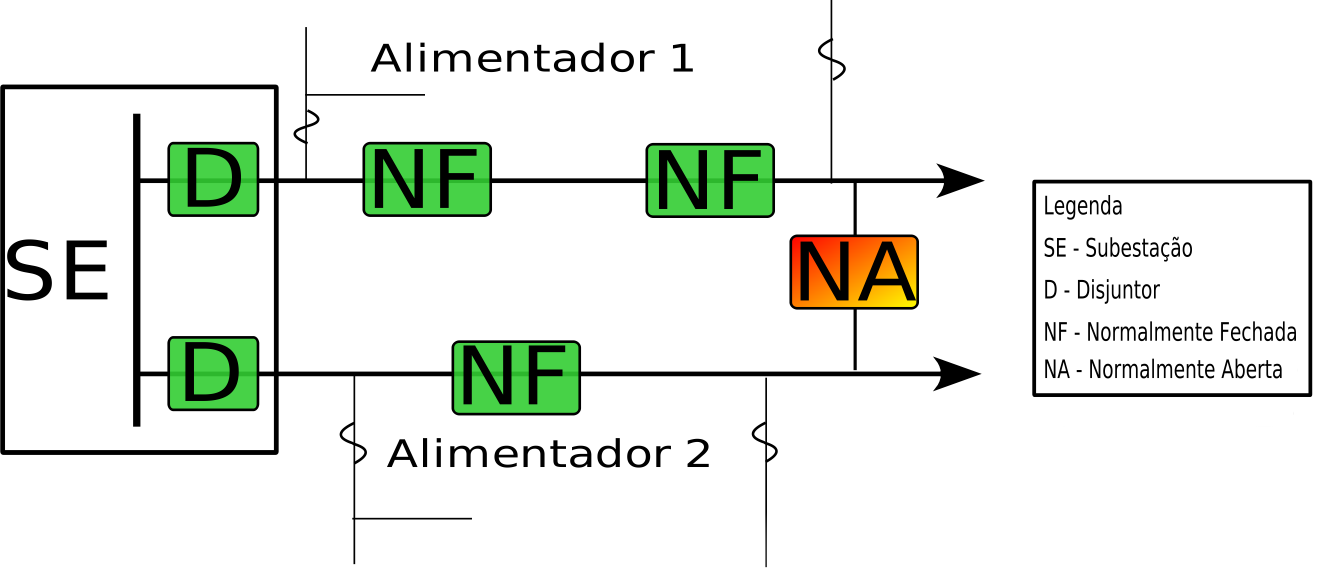
\includegraphics[width=0.8\columnwidth]{img/RedeDist}
\par\end{centering}

\caption{Exemplo de uma Rede Distribui��o Prim�ria \label {fig:redeDistribui��o}}
\end{figure}

Os pontos de carga s�o ou clientes de maior porte, como industrias e grandes centros comerciais, ou transformadores rebaixadores, que reduzem a tens�o para ser ent�o distribu�da pelas redes de distribui��o secund�ria. A energia � transmitida at� esses pontos de carga atrav�s de condutores, os quais possuem caracter�sticas el�tricas que ser�o melhor apresentada no cap�tulo 4, onde ser� explicado o m�todo de simula��o da opera��o das redes de distribui��o.

A rede apresentada (Fig.\ref{fig:redeDistribui��o}) � um modelo de rede de distribui��o radial (que n�o apresenta ciclos) sendo esse modelo muito utilizado nas redes a�reas onde existem postes (de concreto ou madeira) que sustentam os condutores. Esse � um dos diversos modelos poss�veis, sendo outros exemplos as redes subterr�neas do tipo \textit{spot} ou a�reas com prim�rio seletivo \cite{Nelson_Kagan_Introd}, mas que n�o ser�o tratadas desse trabalho. Quando tratamos de redes de distribui��o do tipo radial, alguns termos s�o utilizados para descrever o sentido que a rede est� sendo percorrida: partindo do in�cio do alimentador e percorrendo a rede at� algum ponto de carga, � dito que a rede est� sendo percorrida � jusante; quando a rede � percorrida no sentido de um ponto de carga para o in�cio do alimentador, � dito que se est� percorrendo a rede � montante.


As redes de distribui��o contam com diversos tipos de equipamentos seccionadores, chamados de chaves, sendo alguns deles do tipo de prote��o contra correntes elevadas, origin�rias de defeitos ou sobrecargas, e outros de manobras. Tais equipamentos possuem 2 estados: Aberto quando o fluxo de corrente � interrompida e Fechado caso contr�rio. Tais estados s�o referenciados como NA(normalmente aberto) e NF(normalmente fechado) quando � referenciada o seu estado na topologia original da rede. As chaves permitem que a topologia da rede possa ser seccionada, seja para isolar defeitos ou regi�es para manuten��o, como a troca de condutores ou postes, e tamb�m podem ser utilizados para executar transfer�ncias de parte da carga de um alimentador para outro alimentador, sendo poss�vel diminuir a carga de um alimentador, ou em caso de defeito, restabelecer o fornecimento para parte dos consumidores que se encontram a jusante da �rea afetada. Isto � obtido atrav�s do seccionamento da rede ap�s o defeito e o 
fechamento de alguma chave de fronteira, sendo necess�rio executar simula��es, que ser�o descritas no cap�tulo 4, para verificar se nenhuma parte dos alimentadores ficar� sobrecarregada com a nova topologia da rede.

Normalmente a opera��o de tais chaves de manobra � executada por equipes que devem se deslocar at� a chave para executar a manobra de abertura, quando � desejado que a energia seja interrompida naquele ponto ou de fechamento quando � desejado restabelecer o fluxo a partir daquele ponto. Uma solu��o para evitar esse deslocamento, que pode ser problem�tico em uma cidade grande devido a problemas do tr�nsito, � a automa��o da opera��o de tais equipamentos de manobra.

\section{Automa��o de Sistemas de Distribui��o}
%#Pegar algum livro sobre isso.
Smart Grids
O que � um sistema SCADA
O que � a automa��o de redes? como isso pode ajudar no trabalho (leitura em tempo real dos dados de opera��o e comando remoto das chaves)

\section{Procedimento Convencional para Restabelecimento de Energia El�trica}
Os sistemas de distribui��o est�o sujeitos a condi��es anormais de opera��o, como falha em equipamentos isoladores, descargas el�tricas, contato entre condutores, ou mesmo interfer�ncia no sistema por algum fator externo. Essas condi��es anormais fazem com que os equipamentos de prote��o, atuem para evitar a propaga��o do defeito, tendo como consequ�ncia a interrup��o do fornecimento de energia el�trica para um conjunto de consumidores de um alimentador. 

A rede de distribui��o possui tr�s estados de opera��o \cite{SilvaAloca2010}:
\begin{enumerate}
 \item Estado normal, onde nenhuma restri��o de nenhum equipamento est� violada;
 \item Estado de emerg�ncia, quando acontece um defeito e algum equipamento est� com alguma restri��o violada;
 \item Estado restaurativo, acontece ap�s a atua��o de algum equipamento de prote��o (devido a algum defeito).
\end{enumerate}

No primeiro estado, a rede est� configurada para que nenhum equipamento esteja sobrecarregado e que o m�ximo poss�vel de consumidores estejam com o fornecimento de energia el�trica normalizado. O segundo estado tem in�cio quando acontece algum defeito e pode convergir ao estado normal, sendo apenas um defeito tempor�rio (como um galho de �rvore que tocou em algum condutor) ou o sistema ir� isolar o defeito indo para o estado restaurativo, se o defeito � permanente. Nesse �ltimo estado, o sistema de distribui��o tem um interrup��o parcial ou mesmo total de fornecimento de energia el�trica para os seus consumidores, sendo necess�rio a mobiliza��o de equipes de atendimento para determinar a localiza��o do defeito e logo ap�s executar o seu isolamento e a transfer�ncia de carga para outros alimentadores.

Os religadores, equipamentos de prote��o capazes de atuar para isolar um defeito, ajudam a amenizar os defeitos tempor�rios, uma vez que na ocorr�ncia do defeito o religador atua interrompendo o fornecimento e, depois de alguns instantes, volta a religar a energia se mantendo nesse estado se o defeito n�o existe mais. Normalmente esse ciclo de atua��o e religamento acontece algumas vezes caso o defeito permane�a, sendo interrompido quando o defeito deixar de existir ou o n�mero m�ximo de ciclos tenha acontecido. Quando isso acontece, � dito que o religador entrou em bloqueio e se mant�m no estado aberto (atuado). J� os equipamentos de prote��o como os fus�veis, atuam apenas uma vez quando ocorre algum defeito, n�o voltando a religar ap�s isso.

Quando algum equipamento de prote��o atua ou vai a bloqueio, uma parcela ou mesmo a totalidade dos consumidores ficam com o fornecimento comprometido e se faz necess�rio o trabalho das equipes de manuten��o para detectar e corrigir o problema para que seja poss�vel o restabelecimento total dos consumidores. 

Em alguns casos � poss�vel que o restabelecimento seja parcial atrav�s do isolamento do defeito e transfer�ncia de parte da carga para outros alimentador com uso das chaves existentes nos alimentadores, melhorando com isso a continuidade para alguns consumidores uma vez que eles n�o necessitar�o ficar sem fornecimento de energia el�trica durante todo o tempo de reparo do defeito, mas apenas por uma pequena fra��o de tempo como ser� apresentado a seguir. Considerando a Fig. \ref{fig:exemploDefeito} onde � apresentado um alimentador e um defeito que fez o disjuntor do alimentador atuar no instante $t_0$, seria necess�rio a equipe de manuten��o executar os seguintes passos:
\begin{enumerate}
  \item Localizar o defeito e sua abrang�ncia: isso � feito percorrendo a rede a jusante a partir da chave que atuou.
  \item com o defeito localizado, s�o definidas quais chaves ser�o operadas
  \begin{enumerate}
    \item A chave CH1 � escolhida para ser aberta e assim isolar o defeito do restante da rede a montante
    \item A chave CH2 e NA1 s�o escolhidas para serem manobradas e assim transferir parte para um alimentador vizinho
  \end{enumerate}
  \item A equipe executa as manobras
  \begin{enumerate}
    \item Manobrando a chave CH1 � poss�vel religar a chave atuada restabelecendo os consumidores a montante do defeito, isso � feito no instante $t_1$
    \item A manobra de transfer�ncia usando as chaves CH2 e NA1 � conclu�da no instante $t_2$
\end{enumerate}
 \item O defeito � consertado
 \item As chaves s�o retornadas ao seu estado original no instante $t_3$
\end{enumerate}

\begin{figure}[hb]
\begin{centering}
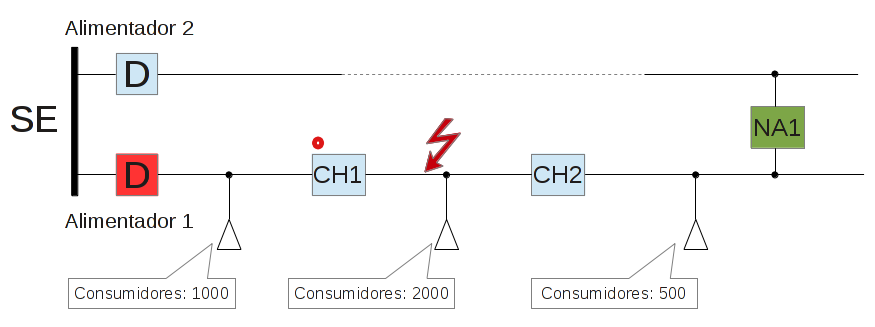
\includegraphics[width=0.8\columnwidth]{img/redeDefeito}
\par\end{centering}
\caption{Rede de Distribui��o Prim�ria com defeito \label{fig:exemploDefeito}}
\end{figure}

Com base nessa sequ�ncia de a��es, � poss�vel concluir que os clientes antes do defeito ficaram sem fornecimento entre $t_0$ e $t_1$ que corresponde ao tempo de localiza��o do defeito, de abertura da chave CH1 e de religamento do disjuntor. Os consumidores ap�s a �rea defeituosa (a jusante da chave CH2) ficaram sem energia el�trica entre os instantes $t_0$ e $t_2$ que corresponde ao tempo de localiza��o do defeito, abertura da chave CH2, deslocamento at� a chave NA1 e seu fechamento. A diferen�a do segundo grupo � que a equipe de manuten��o deve se deslocar ap�s operar a chave CH2 at� a chave NA1, o que n�o � necess�rio no primeiro caso j� que existem operadores na subesta��o para religar o disjuntor. Os demais consumidores na �rea afetada ficaram sem fornecimento entre os instantes de tempo $t_0$ at� o final do conserto e restabelecimento do fornecimento no instante $t_3$, sendo necess�rio o deslocamento entre entre todas as chaves a serem operadas.

Esses tempos s�o chamados de tempo de isolamento, transfer�ncia e de restabelecimento, respectivamente e s�o dados por:
\begin{eqnarray}
T_{i} &=& t_{1} - t_{0}\\
T_{t} &=& t_{2} - t_{0}\\
T_{r} &=& t_{3} - t_{0}
\end{eqnarray}


Onde:
\begin{description}
  \item [$T_i$:] Tempo de isolamento do defeito.
  \item [$T_t$:] Tempo de transfer�ncia de carga.
  \item [$T_r$:] Tempo de restabelecimento total do alimentador.
\end{description}


%\textbf{explicar um pouco melhor o atendimento das equipes, transformar as diferen�as de tempo em $\Delta$}

As interrup��es por causa de defeitos levam a uma diminui��o da continuidade de fornecimento de energia el�trica. A continuidade � medida por indicadores que apresentam o tempo total que um grupo de consumidores ficaram sem fornecimento, al�m da frequ�ncia que os mesmos tiveram o fornecimento interrompido. Tais indicadores s�o definidos por ag�ncias reguladoras, como a ANEEL no Brasil que apresenta tais indicadores com seu respectivos limites no m�dulo 8 do PRODIST \sigla{PRODIST}{Procedimentos de Distribui��o de Energia El�trica no Sistema El�trico Nacional} (Procedimentos de Distribui��o de Energia El�trica no Sistema El�trico Nacional)\cite{prodist2010}. O c�lculo dos indicadores ap�s o defeito apresentado na Fig. \ref{fig:exemploDefeito} � executado usado as f�rmulas  \ref{eq:DEC}, \ref{eq:FEC} para os indicadores globais da rede e \ref{eq:DIC}, \ref{eq:FIC} e \ref{eq:DMIC} para os indicadores individuais de cada unidade consumidora.

DEC:\sigla{DEC} { Dura��o Equivalente por Consumidor } (Dura��o Equivalente por Unidade Consumidora): 
\begin{equation} \label{eq:DEC}
 DEC=\frac{\sum\limits_{i=1}^{k}Ca(i)\cdot t(i)}{Cc}
\end{equation} 

DEC:\sigla{FEC} { Frequ�ncia Equivalente por Consumidor } (Frequ�ncia Equivalente por Unidade Consumidora)
\begin{equation}\label{eq:FEC}
 FEC=\frac{\sum\limits_{i=1}^{k}Ca(i)}{Cc}
\end{equation}
Onde:
\begin{description}
 \item [k] N�mero eventos sendo analisados;
 \item [t(i):] dura��o da interrup��o $i$;
 \item [Ca(i):] N�mero de consumidores afetados pelo evento $i$;
 \item [Cc:] Total de consumidores da rede.
\end{description}

Os indicadores globais oferecem uma �tima vis�o geral da rede em termos de continuidade, apresentando a m�dia de interrup��es por consumidor e o tempo m�dio que cada um deles ficou sem fornecimento de energia el�trica. Apesar disso, os valores podem mascarar situa��o que um pequeno grupo de consumidores ficaram sem energia por um longo per�odo de tempo por exemplo o caso de uma rede que atende 100.000 consumidores e em per�odo o tempo total de interrup��es foi de 100 horas (6000 minutos) e atingiu apenas 100 consumidores, o DEC resultante 6, o que indica que na m�dia cada consumidor ficou 6 minutos sem energia el�trica.


DIC\sigla{DIC} { Dura��o Individual por Consumidor } (Dura��o Individual por Consumidor)
\begin{equation}\label{eq:DIC}
 DIC = \sum_{i=1}^{n}t(i)
\end{equation}

FIC\sigla{FIC} { Frequ�ncia Individual por Consumidor } (Frequ�ncia Individual por Consumidor)
\begin{equation}\label{eq:FIC}
 FIC = n
\end{equation}

DMIC\sigla{DMIC} { Dura��o M�xima Individual por Consumidor } (Dura��o M�xima Individual por Consumidor)
\begin{equation}\label{eq:DMIC}
 DMIC = max_{i=1}^n(t(i))
\end{equation}

Onde:
\begin{description}
  \item [n:] total de interrup��es do cliente;
  \item [t(i):] tempo de interrup��o do evento $i$.
\end{description}

J� os indicadores individuais apresentam uma vis�o focada em apenas um cliente, o que permite identificar pontos cr�ticos como frequ�ncias elevadas de interrup��es e demora para restabelecimento de alguns consumidores.

Considerando as f�rmulas dos indicadores apresentados, a ocorr�ncia do defeito (Fig. \ref{fig:exemploDefeito}) e que os tempos de de isolamento, transfer�ncia e restabelecimento s�o, respectivamente, 10, 20 e 40 minutos, o valor do DEC para o alimentador 1 � apresentado em \ref{eq:DECcalculado}.

\begin{eqnarray}\label{eq:DECcalculado}
DEC_{Alimentador1}&=&\frac{(10 \cdot 1000) + (40 \cdot 2000) + (20 \cdot 500)}{3500}\nonumber\\
&=&\frac{100000}{3500}\nonumber \\
&=&28,57
\end{eqnarray}


Ou seja, cada consumidor ficou cerca de 28,57 minutos sem fornecimento de energia el�trica durante este defeito, que teve dura��o total de 40 minutos. 

Considerando um outro cen�rio, onde o alimentador possui automa��o a n�vel de opera��o das chaves apresentadas, ou seja, um operador pode oper�-las via telecomando, obt�m-se a diminui��o do tempo de opera��o das chaves, uma vez que n�o existir� a necessidade de deslocar equipes entre as chaves, e o conserto pode ser inciado antes.  Para esse cen�rio, se a equipe levar 5 minutos para detectar o defeito, o operador pode executar as manobras de isolamento em tempo real e a de transfer�ncia ap�s alguns poucos minutos, uma vez que isso depende de simula��es para garantir que nenhum tipo de equipamento ficar� sobrecarregado (considerar que na m�dia essas simula��es s�o executadas em 3 minutos), e a equipe j� pode iniciar os trabalhos de reparo da rede. Como pode ser notado, o conserto da rede tem um in�cio mais r�pido, uma vez que a �rea afetado foi isolada em cerca de 8 minutos (5 minutos para detectar mais os 3 minutos de transferir os clientes a jusante do defeito), e tamb�m que tanto os consumidores antes quanto os ap�s o defeito ficaram bem menos tempo sem fornecimento (5 minutos contra os 10 
anteriores para os consumidores � montante do defeito e de 20 para 8 minutos para os � jusante do defeito). Os consumidores da �rea afetada ficaram  no total 28 minutos (8 minutos, do tempo de isolamento total ap�s transfer�ncia dos consumidores a jusante, mais 20 minutos do tempo de reparo do defeito). Com esses novos tempos temos o seguinte c�lculo do DEC desse alimentador:

\begin{eqnarray}\label{eq:DECautomatizado}
DEC_{Alimentador1}&=&\frac{(5 \cdot 1000) + (28 \cdot 2000) + (8 \cdot 500)}{3500}\nonumber\\
&=&\frac{59000}{3500}\nonumber \\
&=&17,57
\end{eqnarray}

Apenas com a automa��o da abertura e fechamento das chaves foi poss�vel reduzir o DEC em quase 11 minutos (cerca de 38\% do tempo anterior). Se considerar o uso de um sistema computacional inteligente que detecte a localiza��o do defeito e defina as chaves a serem manobradas, o tempo pode ser ainda menor, uma vez que a equipe de manuten��o poder� se deslocar para para a �rea defeituosa enquanto o sistema isola a mesma e restabelece o fornecimento em tempo menor ainda.


%\huge{Ver desenho, ver exemplos de manobras, falar sobre os tempos, ETC? }
%\normalsize


% \chapter{Sistemas Computacionais inteligentes}
 Breve introdu��o de sistemas de IA e auxilio na tomada de decis�o


\chapter{Metodologia Proposta}
Modelo do sistema, diagrama de comunica��o,  fluxogramas de tomada de decis�o
% \chapter{Sistema Desenvolvido}

Para validar a metodologia, foi desenvolvido um sistema computacional capaz de representar e simular o funcionamento de uma rede de distribui��o, al�m de permitir a simula��o de defeitos. Dentro desse sistema foi implementada a metodologia apresentada nesse trabalho e funcionalidades que simulam o comportamento dos demais sistemas necess�rios, como o SCADA e hist�rico de carga das redes.

O sistema foi desenvolvido utilizando a linguagem de programa��o C++, a qual oferece robustez e extensibilidade, tendo sido  utilizado o framework Qt \cite{QtSite} para o desenvolvido mais r�pido.


A Fig. \ref{fig:mainWindow} apresenta as principais janelas do sistema. A principal, n�mero 1 � onde s�o apresentadas as mensagens de resposta da metodologia e onde est�o os menus de acesso as op��es.  A janela n�mero 2 permite simular a ocorr�ncia de defeitos. Na parte superior dessa segunda janela, existe um campo o qual cont�m a lista dos disjuntores das redes carregadas. Nesse campo � indicado qual equipamento a metodologia ir� considerar como equipamento desarmado pela corrente de curto circuito. Apesar da lista conter apenas os disjuntores, � poss�vel executar a simula��o de desarme para qualquer equipamento telecomandado das redes carregadas. Os campos pr�-falta e data da falha s�o utilizadas para ajuste de carga, sendo a corrente campo pr�-falta utilizada para o ajuste de carga e a data e hora usada para as simula��es de fluxo de pot�ncia. Os demais campos s�o informa��es que o SCADA iria fornecer em rela��o ao estado do equipamento, tais como como fases sinalizadas (ABCN) e os estados de n�o religar (exclu�do) e controle est� travado (bloqueio). A janela n�mero 3 apresenta algumas op��es da metodologia que podem ser configuradas, como o percentual de sobrecarga dos condutores e dos equipamentos de prote��o, a queda m�xima de tens�o. A quarta janela apenas uma apresenta uma vis�o da topologia da rede carregada.

%%Fig aqui.
\begin{figure}[ht]
\centering
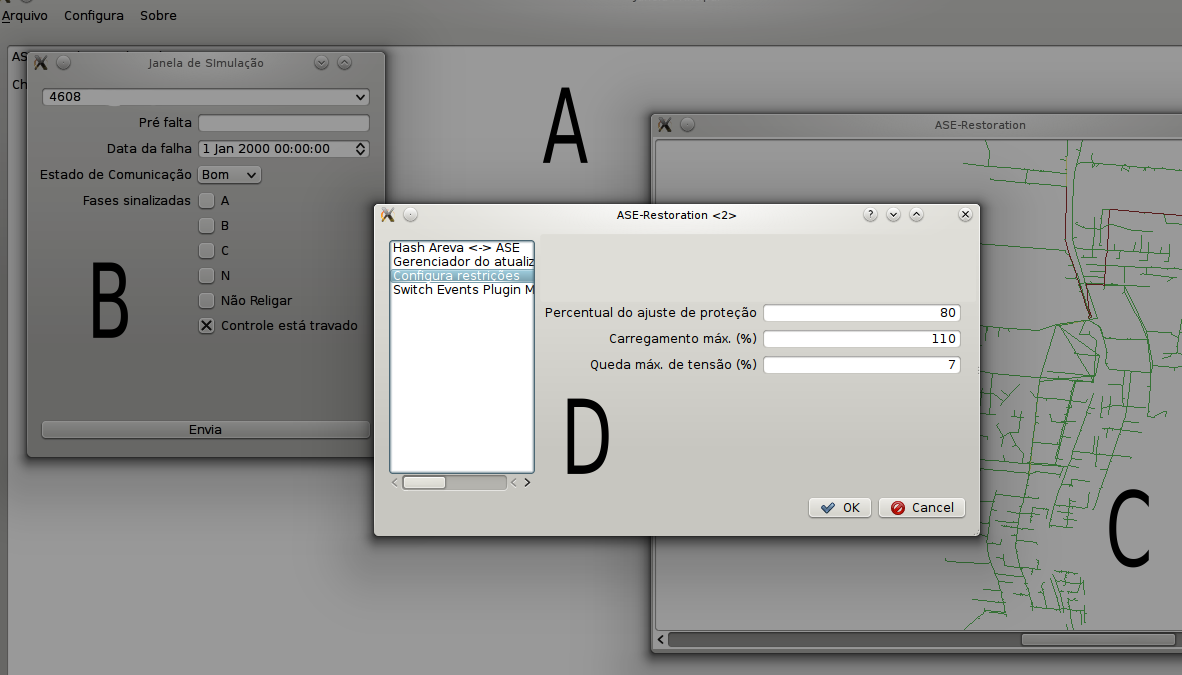
\includegraphics[width=0.8\columnwidth]{img/ASE-Restoration}

\caption{Principais janelas do sistema desenvolvido\label{fig:mainWindow}}

\end{figure}

O envio dessas informa��es � o gatilho de inicio da metodologia apresentada. Caso alguma informa��o estiver incorreta (por exemplo, equipamento de origem n�o � um equipamento telecomandado) o sistema n�o ir� continuar e ir� apresentar uma mensagem na janela principal avisando o motivo de ter interrompido o processamento.

Ap�s o envio das informa��es a serem simuladas, a metodologia necessita atualizar o estado das chaves do alimentador onde o defeito ocorreu e dos alimentadores que fazem fronteira com o mesmo. Para simular esse comportamento, o sistema apresenta uma lista das chaves contidas em tais alimentadores onde � poss�vel mudar o estado das chaves. Isso pode ser visto na Fig \ref{fig:switchStatus}, onde as chaves marcadas s�o as que ao final ter�o o estado Fechado e as n�o marcadas ter�o o estado Aberto. Caso alguma opera��o de fechar leve a um ciclo na rede (lembrando que uma restri��o � a radialidade do sistema), a metodologia � interrompido e uma mensagem � indicada na janela principal.

%%Fig Aqui.
\begin{figure}[ht]
\centering
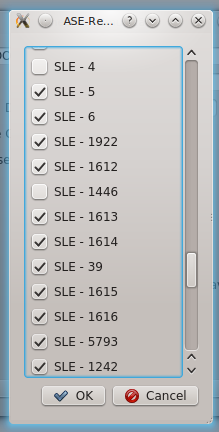
\includegraphics[width=0.2\columnwidth]{img/EstadoChaves}

\caption{Requisi��o do estado das chaves.\label{fig:switchStatus}}

\end{figure}

Com o estado das chaves atualizados, a metodologia define a lista de equipamentos que podem ser utilizados para o restabelecimento autom�tico e agora necessita obter mais informa��es sobre tais equipamentos, para s� ent�o executar as simula��es. Para equipamento que poder� ser utilizado, o sistema apresenta a janela da Fig \ref{fig:switchSCADARequest}, onde s�o solicitadas as informa��es do estado atual do equipamento telecomandado. As informa��es solicitadas s�o o estado (Aberto/Fechado) da chave, a exist�ncia da sinaliza��o da passagem da corrente de curto por alguma fase, o estado de comunica��o, se a chave est� exclu�da (n�o religar) e se o equipamento est� em bloqueio. Tamb�m � solicitada a corrente pr�-falta de cada equipamento, mas esse valor somente � considerado para os disjuntores dos alimentadores.

%%Fig Aqui
\begin{figure}[ht]
\centering
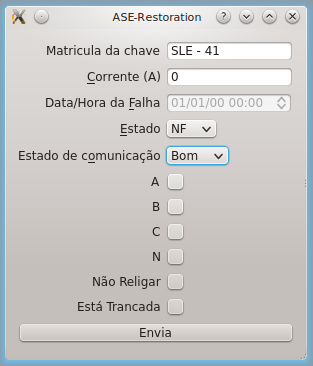
\includegraphics[width=0.3\columnwidth]{img/SwitchSCADARequest}

\caption{Requisi��o das informa��es de um equipamento telecomandado.\label{fig:switchSCADARequest}}

\end{figure}

Nesse ponto o sistema j� disp�e de todas informa��es necess�rias para executar as simula��es, tanto de opera��o da rede quanto das manobras de isolamento e transfer�ncia de carga. Como resultado � obtida uma sequ�ncia de manobras que podem ser executadas, na qual s�o inclu�das as manobras que violam as restri��es, sendo que as �ltimas o sistema n�o as coloca como execut�veis. A Fig \ref{fig:maneuversWindows} apresenta um exemplo de manobras que contemplam o isolamento de defeitos (chave 5103) e a transfer�ncia (SLE - 47), sendo que a �ltima n�o est� marcada para execu��o por existirem restri��es em um equipamento de prote��o (5203 com 90.62\% de carga). Nessa �ltima janela � poss�vel aplicar as manobras (inclusive as que est�o com algum tipo de sobrecarga), bastando marcar as manobras e clicar e Ok. Essa aplica��o das manobras � �til para simular a ocorr�ncia de novos defeitos quando a rede se encontra em estado de conting�ncia.


%%fig Aqui
\begin{figure}[ht]
\centering
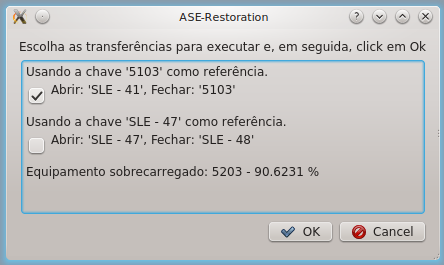
\includegraphics[width=0.4\columnwidth]{img/maneuversOptions}

\caption{Op��es de manobras simuladas.\label{fig:maneuversWindows}}

\end{figure}







% \chapter{Resultados Pr�ticos \label{cap:casosestudos}}
% Apresentar algumas topologias de estudo, mostrar resultados preliminares com o Rocs para o sistema de teste, mostrar algumas redes (pedir permiss�o para a AES?)

Para validar a metodologia e analisar os resultados gerados pela mesma, foram executados testes e simula��es de defeitos em redes de distribui��o reais. As simula��es consideraram a ocorr�ncia de defeitos antes, depois e entre equipamentos telecomandados tentando criar uma variedade de cen�rios de defeitos. Tamb�m foram executadas simula��es em diferentes hor�rios para analisar o comportamento da metodologia em diferentes patamares de carga.

Para avaliar e validar o algoritmo de busca de manobras, foi implementado um prot�tipo utilizando a ferramenta Rocs \cite{Rocs2012}. O Rocs � uma ferramenta de pesquisa em Teoria de Grafos que permite visualizar e interagir utilizando algoritmos escritos em linguagem Javascript\footnote{Linguagem de programa��o. Muito utilizada para programa��o em tempo de execu��o.}.

Ap�s esses estudos e refinamentos iniciais do funcionamento do algoritmo de busca, foi desenvolvida uma ferramenta computacional para a simula��o da opera��o de redes de distribui��o e tamb�m a simula��o da ocorr�ncia de defeitos. A descri��o do sistema desenvolvido se encontra na se��o \ref{sistemaDesenvolvido}.

A Figura \ref{fig:ExemploredeRocs} ilustra a tela inicial do Rocs com um representa��o simplificada de uma rede de distribui��o, onde os n�s em cor azul representam os equipamentos telecomandados NF (normalmente fechado) e os de
cor vermelha os equipamentos NA (normalmente abertos). Tamb�m h� a indica��o
dos valores de carga em cada trecho, sendo que nas simula��es foi considerado que qualquer transfer�ncia pode ser executada contanto que a carga total de tal transfer�ncia n�o ultrapasse 100 UC\footnote{Optou-se por n�o usar Amperes pois n�o existe uma simula��o da rede, apenas um valor de carregamento arbitr�rio.} (Unidades de Carregamento). Foi considerado que todos os trechos entre os equipamentos possuem o mesmo n�mero de consumidores, assim quanto mais o n�mero de trechos transferidos maior o n�mero de consumidores restabelecidos.

\begin{figure}[htbp]
\centering
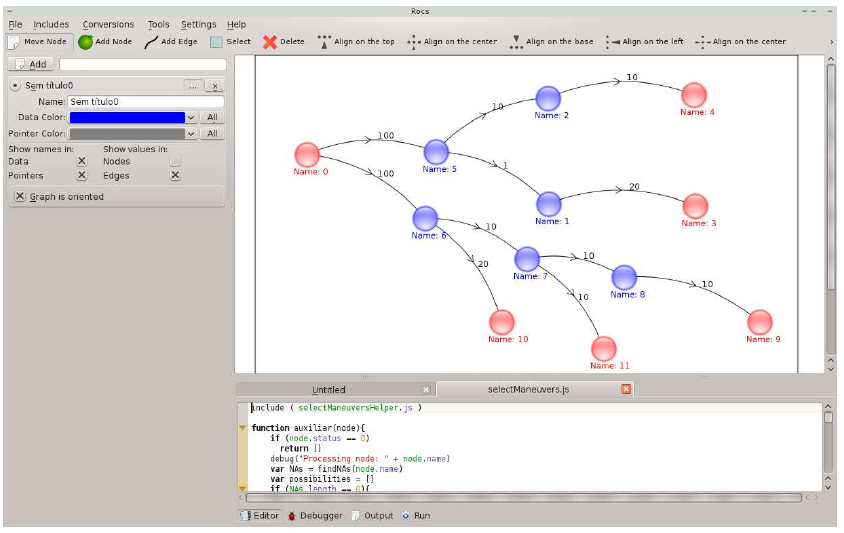
\includegraphics[width=0.8\columnwidth]{img/rocsTela1}
\caption{Topologia inicial do caso de teste.\label{fig:ExemploredeRocs}}
\end{figure}

Para ilustrar a aplica��o do algoritmo de sele��o de chaves para transfer�ncia, ser�o apresentados dois estudos de
casos. No primeiro caso, considerou-se o defeito ap�s o equipamento ``0'', ou seja, nos trechos ``0 - 5'' e ``0 - 6'', e
analisou-se as transfer�ncias de carga realizadas pela metodologia proposta. Para o
defeito no trecho ``0 - 5'', o sistema abriu o equipamento ``5'', isolando o
defeito, e fechou o equipamento ``3'', restabelecendo a energia para as cargas
a jusante do defeito. J� para o defeito no trecho ``0 - 6'', o sistema abriu o
equipamento ``6``, isolando o defeito, e fechou o equipamento  ``10'',
restabelecendo a energia para as cargas a jusante do defeito. A figura \ref{fig:ResultadoRocs1} apresenta a topologia final ap�s essas manobras.

\begin{figure}[htbp]
\centering
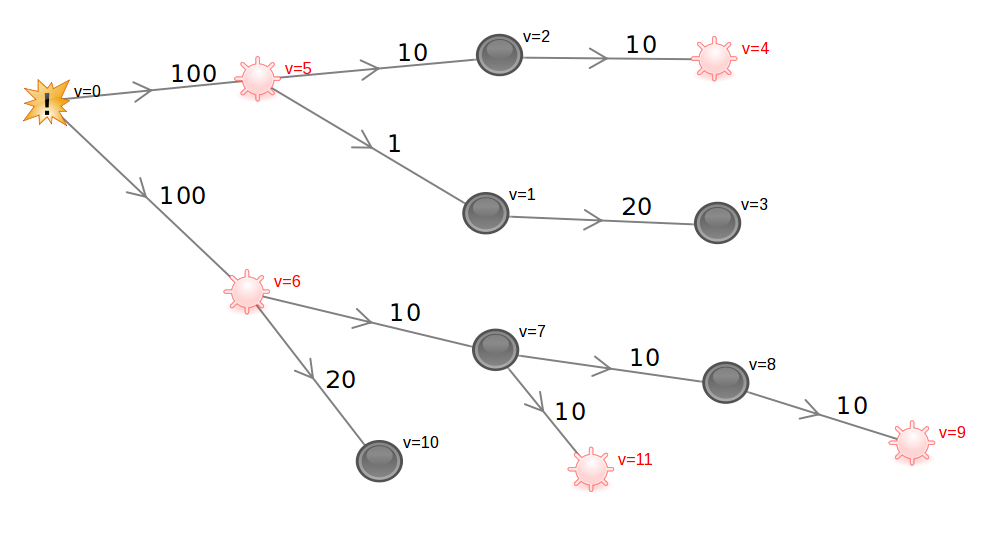
\includegraphics[width=0.8\columnwidth]{img/rocsTela2}
\caption{Resultado do estudo do caso 1.\label{fig:ResultadoRocs1}}
\end{figure}

No segundo caso aumentou-se os valores de corrente no trecho ``5 - 1'' de 1 para 80 e no trecho ``8 - 9'' de 10 UC para 90 UC. Nesse novo cen�rio, a resposta oferecida anteriormente deixa de ser v�lida, uma vez que a carga total seria de 120 UC no equipamento ``3'' e 140 UC no equipamento ``10''. A proposta desse segundo caso � verificar se o sistema realizar� mais do que uma manobra para transferir
as cargas a jusante do defeito, isto �, se dividir� as cargas entre diferentes equipamentos NA
 para que nenhum deles venha a violar a restri��o definida.

De acordo com a Figura \ref{fig:ExemploredeRocs2} verifica-se que a metodologia respondeu de
forma satisfat�ria. Para o defeito no trecho ``0 - 5'', o sistema abriu os equipamentos
dos n�s ``5'' e ``1'', fechando os n�s ``4'' e ``3'', de modo a transferir parte da carga para
um dos equipamentos de fronteira e parte para o outro, evitando assim a viola��o da restri��o, j� que o equipamento ``4'' recebeu 100 UC  e o ``3'' recebeu 20 UC. J� para
o defeito no trecho ``0 - 6'', o sistema abriu os equipamentos dos n�s ``6'' e ``8'',
fechando os n�s ``10'' e ``9'', de modo a transferir parte da carga para um alimentador
e parte para o outro, evitando assim a viola��o da restri��o uma vez que o equipamento ``9'' recebeu 90 UC e o equipamento ``10'' recebeu 50 UC.

\begin{figure}[htbp]
\begin{centering}
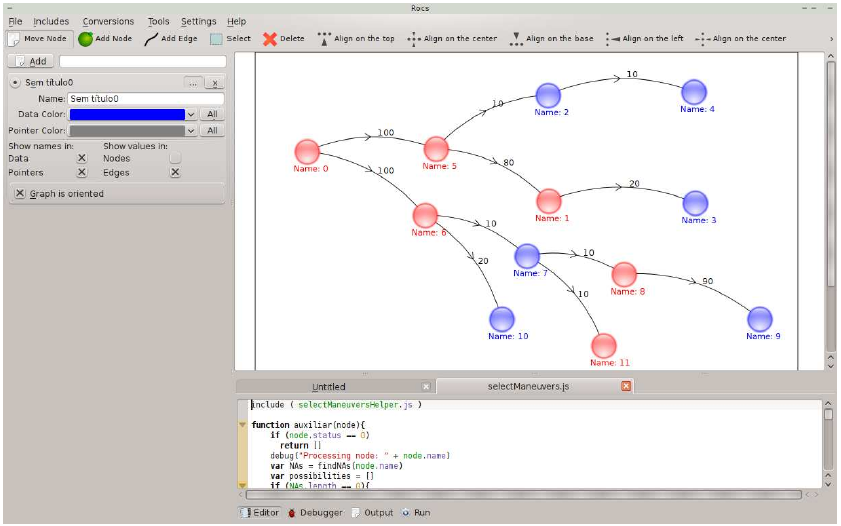
\includegraphics[width=0.8\columnwidth]{img/rocsTela3}
\par\end{centering}
\caption{Resultado do estudo do caso 2.\label{fig:ExemploredeRocs2}}
\end{figure}


\section{Sistema Desenvolvido\label{sistemaDesenvolvido}}

Para validar a metodologia completa, foi desenvolvido um sistema computacional capaz de representar e simular o funcionamento de uma rede de distribui��o, al�m de permitir a simula��o de defeitos. Para isso, esse sistema implementa  as funcionalidades de simula��o dos componentes citados como o SCADA, hist�rico de carga das redes al�m do algoritmo de escolha de manobras.

O sistema foi desenvolvido utilizando a linguagem de programa��o C++ por oferecer robustez e extensibilidade, tendo sido  utilizado o framework Qt \cite{QtSite} para o desenvolvido mais r�pido, uma vez que o mesmo j� disponibiliza componentes gr�ficos e alguns padr�es de design j� implementados.


A Fig. \ref{fig:mainWindow} apresenta as principais janelas do sistema. A janela principal (\ref{fig:mainWindow}-A) � onde s�o apresentadas as mensagens de resposta da metodologia e onde est�o os menus de acesso �s op��es.  A janela de simula��o de eventos (\ref{fig:mainWindow}-B) permite simular o envio de eventos de desarme dos equipamentos. Na parte superior dessa janela, existe um campo no qual � indicado qual equipamento a metodologia ir� considerar como equipamento desarmado pela corrente de curto-circuito. Apesar da lista conter inicialmente apenas os disjuntores, � poss�vel executar a simula��o de desarme para qualquer equipamento telecomandado das redes carregadas. A corrente do campo pr�-falta � utilizada para o ajuste de carga e a data e hora usada para as simula��es de fluxo de pot�ncia. Os demais campos s�o informa��es em rela��o ao estado do equipamento, tais como fases sinalizadas (ABCN) e os estados de n�o religar
(exclu�do) e se o controle est� travado (bloqueio). A janela D (\ref{fig:mainWindow}-D) apresenta algumas op��es da metodologia que podem ser configuradas, como o percentual de sobrecarga dos condutores e dos equipamentos de prote��o, e a queda m�xima de tens�o. A �ltima janela (\ref{fig:mainWindow}-C) � apenas uma visualiza��o da topologia da rede carregada.

%%Fig aqui.
\begin{figure}[ht]
\centering
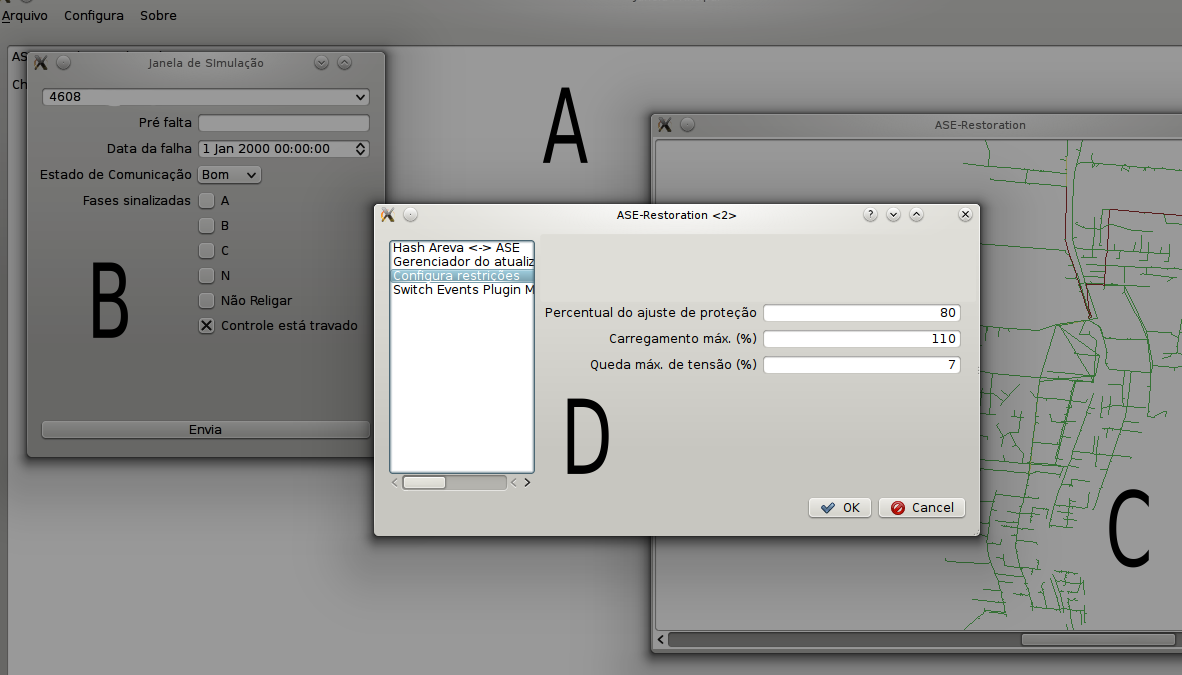
\includegraphics[width=0.9\columnwidth]{img/ASE-Restoration}

\caption[Principais janelas do sistema desenvolvido]{Principais janelas do sistema desenvolvido\\A) Janela principal,\\B) Janela de simula��o de eventos,\\C) Visualiza��o das redes carregadas,\\D) Configura��es de restri��es.\label{fig:mainWindow}}

\end{figure}

O envio dessas informa��es � o gatilho de in�cio da metodologia apresentada. Caso alguma informa��o estiver incorreta (por exemplo, equipamento de origem n�o � um equipamento telecomandado) o sistema n�o ir� continuar e ir� apresentar uma mensagem na janela principal avisando o motivo de ter interrompido o processamento.

Ap�s o envio das informa��es para simula��o, a metodologia necessita atualizar o estado das chaves do alimentador onde o defeito ocorreu e dos alimentadores que fazem fronteira com o mesmo. Para simular esse comportamento, o sistema apresenta uma lista das chaves contidas em tais alimentadores onde � poss�vel mudar o estado das chaves. Isso pode ser visto na Fig \ref{fig:switchStatus}, onde as chaves marcadas s�o as que ao final ter�o o estado Fechado e as n�o marcadas ter�o o estado Aberto. Caso alguma opera��o de fechar um equipamento forme um anel na rede (lembrando que uma restri��o � a radialidade do sistema), a metodologia � interrompida e uma mensagem � exibida na janela principal.

%%Fig Aqui.
\begin{figure}[htbp]
\centering
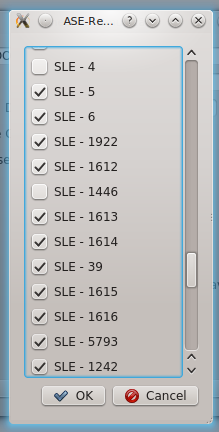
\includegraphics[width=0.16\columnwidth]{img/EstadoChaves}

\caption{Requisi��o do estado das chaves.\label{fig:switchStatus}}

\end{figure}

Com o estado das chaves atualizado, a metodologia define a lista de equipamentos que podem ser utilizados para o restabelecimento autom�tico e agora necessita obter mais informa��es sobre tais equipamentos, para s� ent�o executar as simula��es. Para cada equipamento que poder� ser utilizado, o sistema apresenta a janela da Fig \ref{fig:switchSCADARequest}, onde s�o solicitadas as informa��es do estado atual do equipamento telecomandado. As informa��es solicitadas s�o o estado (Aberto/Fechado) da chave, a exist�ncia da sinaliza��o da passagem da corrente de curto-circuito por alguma das fases, o estado de comunica��o, se a chave est� exclu�da (n�o religar) e se o equipamento est� em bloqueio. Tamb�m � solicitada a corrente pr�-falta de cada equipamento, por�m esse valor somente � considerado para os disjuntores dos alimentadores.

%%Fig Aqui
\begin{figure}[htbp]
\centering
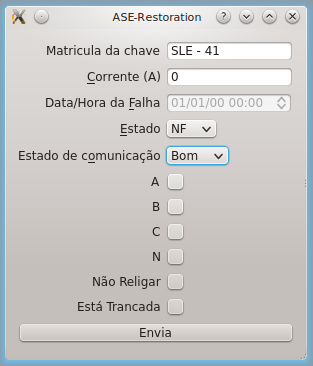
\includegraphics[width=0.27\columnwidth]{img/SwitchSCADARequest}

\caption{Requisi��o das informa��es de um equipamento telecomandado.\label{fig:switchSCADARequest}}

\end{figure}

Nesse ponto o sistema j� disp�e de todas informa��es necess�rias para executar as simula��es, tanto de opera��o da rede quanto das manobras de isolamento e transfer�ncia de carga. Como resultado � obtida uma sequ�ncia de manobras que podem ser executadas, na qual s�o inclu�das as manobras que violam as restri��es, sendo que estas o sistema n�o coloca como execut�veis.

A Fig \ref{fig:maneuversWindows} apresenta uma poss�vel solu��o para um defeito simulado. As manobras ali apresentadas, contemplam o isolamento de defeitos (chave 5103) e a transfer�ncia (SLE - 47), sendo que a �ltima n�o est� marcada para execu��o por existirem restri��es em um equipamento de prote��o (5203 com 90.62\% de carga). Nessa �ltima janela � poss�vel aplicar as manobras (inclusive as que est�o com algum tipo de sobrecarga), bastando marcar as manobras e clicar em \textit{Ok}. Essa aplica��o das manobras � �til para simular a ocorr�ncia de novos defeitos quando a rede se encontra em estado de conting�ncia. Mais informa��es sobre cada uma das transfer�ncias s�o apresentadas na janela principal.


%%fig Aqui
\begin{figure}[htbp]
\centering
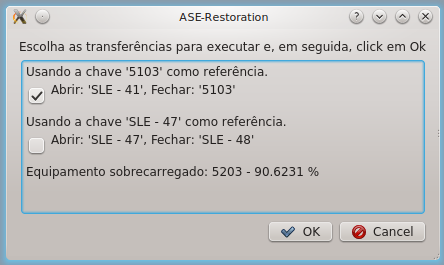
\includegraphics[width=0.4\columnwidth]{img/maneuversOptions}

\caption{Op��es de manobras simuladas.\label{fig:maneuversWindows}}

\end{figure}

Com a ferramenta desenvolvida e as simula��es de fluxo de pot�ncia e controle de carga por curvas t�picas previamente validadas, foram executados diversos casos de teste, os quais est�o descritos na pr�xima se��o.

\section{Resultados Obtidos}

Com esses estudos preliminares e o desenvolvimento da ferramenta computacional a metodologia foi aplicada em rede reais maiores, como por exemplo a apresentada na Figura \ref{fig:Rede-testes}, onde o n�mero de equipamentos � maior e a disposi��o � diferente para cada rede, uma vez que s�o diferentes topologias para cada alimentador.

\begin{figure}[htbp]
\centering
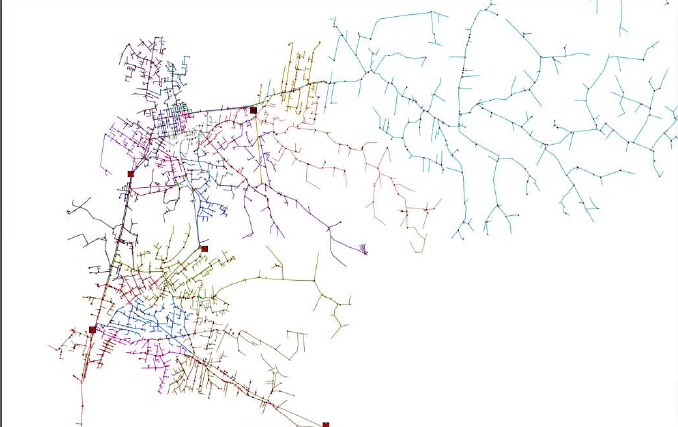
\includegraphics[width=0.85\columnwidth]{img/redeDeTestes}

\caption{Representa��o da rede escolhida para aplica��o dos testes\label{fig:Rede-testes}}

\end{figure}

As redes representadas graficamente na Figura \ref{fig:Rede-testes} foram as redes escolhidas para realizar os casos de teste. Elas s�o redes reais de uma concession�ria do Rio Grande do Sul e possuem 132.890 consumidores e um total de 41 equipamentos telecomandados distribu�dos entre seus 21 alimentadores. Uma vis�o simplificada dos alimentadores e alguns equipamentos telecomandados est� apresenta no diagrama unifilar da Figura \ref{fig:Unifilar-Rede-Testes}.


\begin{figure}[htbp]
\centering
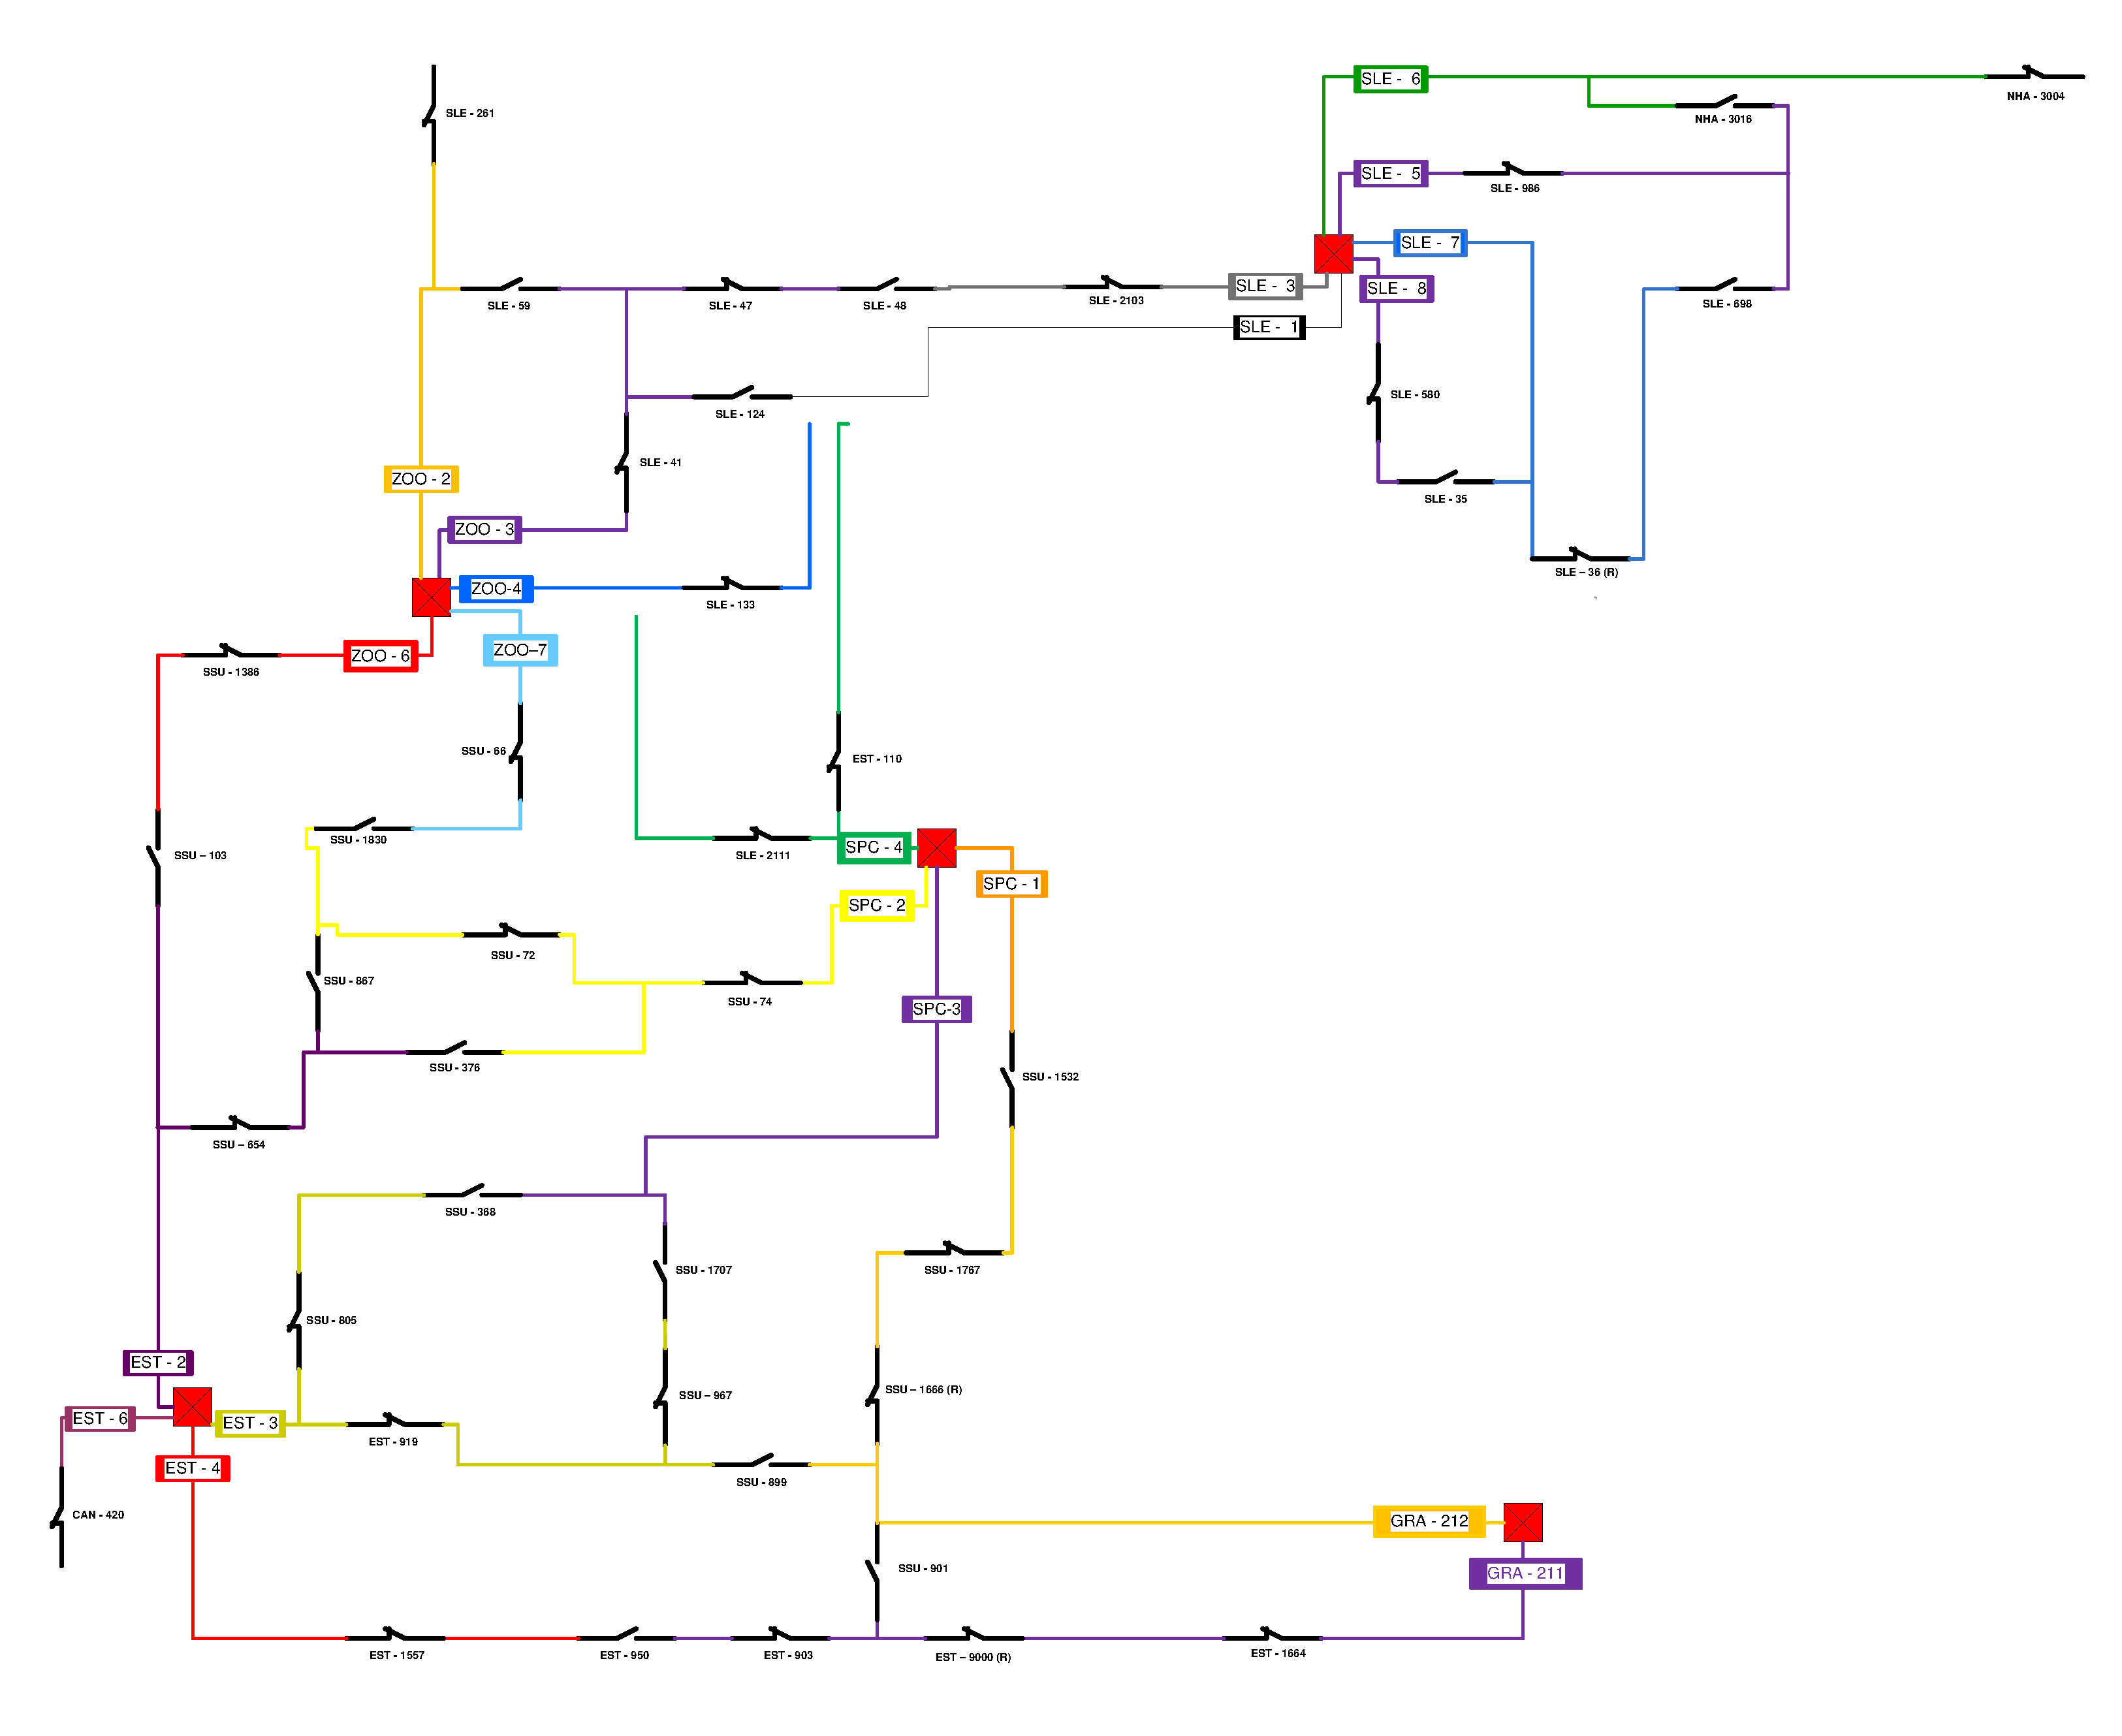
\includegraphics[width=0.9\columnwidth]{img/Unifilar-Com_Nomes}

\caption{Representa��o unifilar da rede de testes\label{fig:Unifilar-Rede-Testes}}
\end{figure}

Nessas redes foram executadas simula��es de defeito em diferentes pontos, antes e ap�s equipamentos telecomandados, atrav�s do envio de desarmes com bloqueio dos equipamentos. Tamb�m foi executado o teste de equipamentos sinalizados pela corrente de curto, ou seja, casos onde o defeito se encontrava a montante do equipamento sinalizado, por exemplo por n�o estar programado para agir como equipamento de prote��o. A se��o seguinte apresenta os resultados desses testes indicando as manobras sugeridas e informa��es, como consumidores restabelecidos, carregamento e queda de tens�o, de cada uma dessas op��es.



% Mostrar alguns resultados de redes reais. Necess�rio casos fict�cios?

Para executar os casos de testes foram consideradas as restri��es de carregamento m�ximo dos equipamentos de prote��o de 90\%, carregamento m�xima dos condutores de 110\% e queda m�xima de tens�o de 7\%.
Os testes aqui apresentados foram definidos de modo a contemplar as poss�veis topologias e demostrar que as escolhas feitas pela metodologia s�o as melhores entre as aceit�veis, ou seja, dentre as que n�o violam nenhuma restri��o s�o escolhidas as que restabelecem o maior n�mero de consumidores. Para os casos onde a metodologia n�o apresentou nenhuma solu��o, s�o apresentadas as manobras poss�veis e s�o indicadas as restri��es violadas.

\subsection[Caso 1]{Caso 1: Transfer�ncia de carga simples para alimentador vizinho}
Os primeiros casos de teste consideram apenas um equipamento telecomandado no alimentador mais um de fronteira que pode ser utilizando para executar transfer�ncias. A Figura \ref{fig:Unifilar-Caso1} apresenta o alimentador escolhido para os primeiros testes.

\begin{figure}[htbp]
\centering
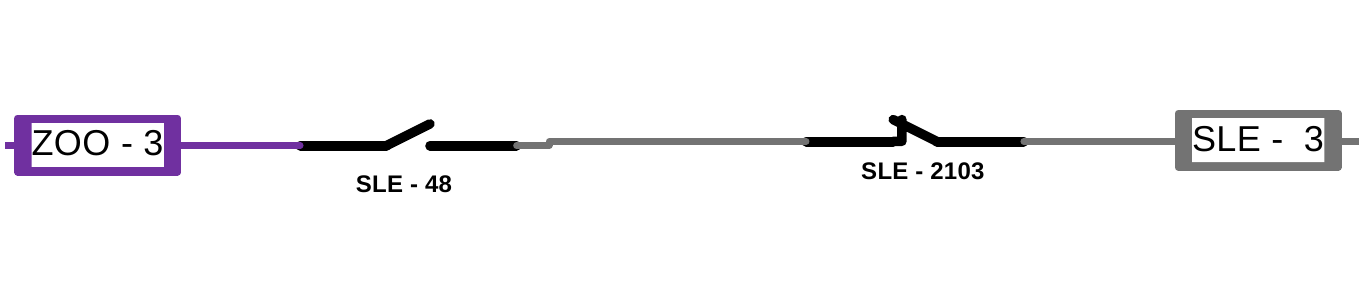
\includegraphics[width=0.7\columnwidth]{img/Caso1Unifilar}

\caption[Representa��o unifilar para casos 1,2 e 3]{Representa��o unifilar dos alimentadores envolvidos no caso de teste N� 1, 2 e 3\label{fig:Unifilar-Caso1}}
\end{figure}

O primeiro teste realizado foi a simula��o do desarme do disjuntor do alimentador ``SLE - 3'' sem a sinaliza��o de passagem de corrente de curto-circuito em nenhum outro equipamento telecomandado. Analisando a topologia apresentada, � poss�vel deduzir que, como o defeito n�o foi detectado (sinaliza��o de alguma fase) por nenhum equipamento a n�o ser o disjuntor, o defeito se encontra no primeiro trecho (entre a sa�da do alimentador  e o equipamento ``SLE - 2103''). Quando o disjuntor desarmou, todos os consumidores do alimentador ``SLE - 3'' ficaram sem fornecimento de energia el�trica. Na rede apresentada existe um equipamento de fronteira (``SLE - 48'') que pode ser utilizado em conjunto com a chave ``SLE - 2103'' para transferir os clientes situados ap�s o defeito para o alimentador vizinho (ZOO - 3). O resultado esperado da metodologia � que ele indique a chave ``SLE - 2103'' para ser aberta e a chave ``SLE - 48'' para ser fechada, se isso n�o violar nenhuma das restri��es impostas. Num primeiro
instante a
metodologia indicou que existia um equipamento sobrecarregado e que a manobra n�o poderia ser executada, como pode ser visto nos resultados apresentados na Tabela \ref{caso1-Sobrecarga}.

\begin{table}[htbp]
\caption{Resultados caso de teste 1 - Cadastro original da rede}
\begin{tabular}{|c|c|c|r|r|r|r|}
\hline
Manobra & Abrir & Fechar & Clientes & Condutores (\%) & Prote��o (\%) & Queda (\%) \\ \hline
\multicolumn{1}{|c|}{$1^\dag$} & \multicolumn{1}{c|}{SLE - 2103} & \multicolumn{1}{c|}{SLE - 48} & \multicolumn{1}{r|}{1867} & \multicolumn{1}{r|}{47,2635} & \multicolumn{1}{r|}{2203,83} & \multicolumn{1}{r|}{0,8358} \\ \hline
\end{tabular}
\label{caso1-Sobrecarga}
\end{table}

Antes de analisar a tabela contendo os resultados, segue uma breve explica��o sobre seu conte�do. Nas tabelas de resultado da metodologia cada linha representa uma manobra que a metodologia considerou. Para quest�o compara��o, mesmo as manobras que apresentaram restri��es violadas ser�o apresentadas. 

Cada linha possui um n�mero na coluna \textit{Manobra} e � composta por um equipamento que deve ser aberto, indicado na coluna \textit{Abrir}, e um que deve ser fechado, coluna \textit{Fechar}. A coluna \textit{Clientes} indica quantos clientes a manobra ir� restabelecer se  for executada. As tr�s colunas restantes s�o as indica��es dos percentuais de carregamento m�ximo  de condutores na coluna Condutores, de carregamento m�ximo dos equipamentos de prote��o na coluna Prote��o e o percentual m�ximo de queda de tens�o na coluna Queda. As manobras que violam alguma das restri��es possuem uma marca ($^\dag$) ao lado no n�mero da manobra. J� as manobras indicadas pela metodologia como podendo ser aplicadas 
diretamente possuem a marca \textdegree.


Analisando o resultado da Tabela \ref{caso1-Resultados}, a manobra apresentada � a esperada, mas como pode ser visto na coluna Prote��o, que indica o percentual m�ximo de carga nos equipamentos de prote��o, o valor 2203,83\% indicado � muito superior a restri��o de 90\% definida anteriormente, por isso ela n�o foi indicada para ser executada. Ao analisar a rede, foi notada a exist�ncia de um poss�vel erro de cadastro. Um equipamento de prote��o possu�a capacidade m�xima de 3A sendo que a corrente m�dia simulada, em regime normal de opera��o, era de 50A. 

Ap�s acertar o ajuste desse equipamento para uma corrente superior (100A), a metodologia apresentou os resultados na Tabela \ref{caso1-Resultados} e indicou que a manobra poderia ser executada de forma autom�tica, ou seja, os comandos de abertura e fechamento dos equipamento poderiam ser enviados para o SCADA execut�-los.

\begin{table}[htbp]
\caption{Resultados para o caso de teste 1}
\begin{tabular}{|c|c|c|r|r|r|r|}
\hline
Manobra & Abrir & Fechar & Clientes & Condutores (\%) & Prote��o (\%) & Queda (\%) \\ \hline
1\textdegree & SLE - 2103 & SLE - 48 & \multicolumn{1}{r|}{1867} & \multicolumn{1}{r|}{47,2635} & \multicolumn{1}{r|}{46,5248} & \multicolumn{1}{r|}{0,8358} \\ \hline
\end{tabular}
\label{caso1-Resultados}
\end{table}

A manobra sugerida poderia inicialmente restabelecer 1867 consumidores, isolando o defeito sem a necessidade do deslocamento de nenhuma equipe para executar essa manobra, liberando-as para se concentrarem em solucionar rapidamente o defeito da �rea sem fornecimento ou mesmo executando mais manobras para transferir mais consumidores. %Os resultados desse primeiro caso de teste foram bom para ver que a metodologia � capaz de evitar sobrecargas no sistema de distribui��o.

\subsection[Caso 2]{Caso 2: Isolamento simples}


No segundo caso teste, a regi�o do defeito foi modificada para a regi�o ap�s a chave ``SLE - 2103''. Os eventos enviados como entrada na metodologia foram o desarme do disjuntor do alimentador ``SLE - 3'' e a sinaliza��o da passagem da corrente de curto-circuito pelo equipamento ``SLE - 2103''. O esperado da metodologia � que ela indique uma manobra que isole o fornecimento de energia ao defeito, utilizando a chave ``SLE - 2103'', de modo que o disjuntor possa ser religado novamente. 

O resultado obtido pela metodologia est� descrito na Tabela \ref{caso2-Resultados}, onde pode ser visto que a metodologia apresentou o resultado esperado. Pode-se notar que n�o existem valores de carregamentos e queda de tens�o, uma vez que essa manobra apenas restabelece o fornecimento de energia el�trica para uma regi�o que antes era alimentada tendo como �nica diferen�a a redu��o da �rea de fornecimento em rela��o a topologia antes do defeito.
% consumidores, assim se n�o

\begin{table}[htbp]
\caption{Resultados para o caso de teste 2}
\begin{tabular}{|c|c|c|r|r|r|r|}
\hline
Manobra & Abrir & Fechar & Clientes & Condutores (\%) & Prote��o (\%) & Queda (\%) \\ \hline
1\textdegree & SLE - 2103 & 5103 (disjuntor) & \multicolumn{1}{r|}{7} & - & - & - \\ \hline
\end{tabular}
\label{caso2-Resultados}
\end{table}

\subsection[Caso 3] {Caso 3: Defeito j� isolado, sem op��es de manobras}
O terceiro caso de teste � uma varia��o do caso 2 caso de teste � quando o equipamento ``SLE - 2103'' est� configurado como equipamento de prote��o, ou seja, na ocorr�ncia de uma corrente de curto-circuito o mesmo atua para interromper o fluxo de corrente. Nesse caso como o defeito aconteceu a jusante do equipamento, ele ir� atuar e isolar o defeito. 

Como n�o existe nenhum outro equipamento NF ap�s o defeito  que possa ser usado para transferir parte da carga para outro alimentador, n�o existe nenhuma manobra que possa ser executada utilizando os equipamentos telecomandados e a metodologia n�o apresenta nenhuma resposta, o que era o esperado.

Os casos apresentados at� aqui visavam testar se a metodologia era capaz de realizar as opera��es simples de isolamento e transfer�ncia de carga de forma autom�tica

\subsection [Caso 4] {Caso 4: Transfer�ncia e isolamento simult�neos}
Os pr�ximos casos de testes envolvem diversas possibilidades de transfer�ncia para diferentes alimentadores e o uso de isolamento e transfer�ncia juntas para restabelecer o maior n�mero de consumidores. As redes escolhidas para teste apresentam mais de um equipamento telecomandado em s�rie e fronteira com mais de uma alimentador.

O caso de teste 4 envolver� as redes apresentadas na Figura \ref{fig:Unifilar-Caso4}, tendo como objetivo verificar se a metodologia � capaz de isolar e transferir carga para um alimentador vizinho ao mesmo tempo, para isso ser� simulada a ocorr�ncia de um defeito no trecho entre os equipamentos ``SLE - 74'' e ``SLE - 72'' que levou ao disjuntor do alimentador ``SPC - 2'' desarmar.

\begin{figure}[htbp]
\centering
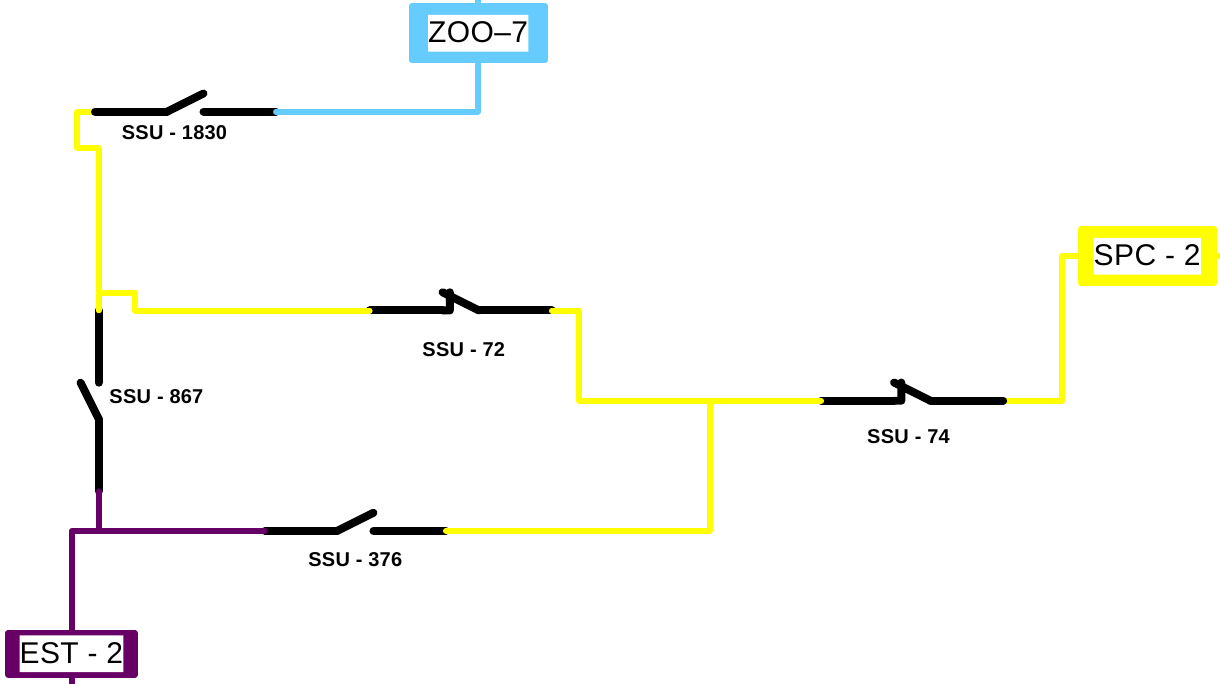
\includegraphics[width=0.7\columnwidth]{img/Caso3Unifilar}

\caption[Representa��o unifilar para os casos 4 e 5]{Representa��o unifilar dos alimentadores envolvidos nos casos de teste 4 e 5\label{fig:Unifilar-Caso4}}
\end{figure}

Como o defeito foi a jusante do equipamento ``SLE - 74'' e o mesmo n�o desarmou com a passagem da corrente de curto-circuito, ele � sinalizado para a metodologia como tendo sido atravessado por tal corrente. Com as informa��es do estado atual das demais chaves, a metodologia apresentou as manobras da Tabela \ref{caso3-Resultados}, onde a manobra 1 � de isolamento, que ser� indicada para ser executada, e as manobras 2 e 3 s�o duas op��es distintas de transfer�ncia, sendo que a apresentada pela metodologia para ser executada automaticamente foi a manobra 3, que apesar de ter um carregamento maior nos equipamentos de prote��o, possui um carregamento menor dos condutores da rede.

\begin{table}[htbp]
\caption{Resultados para o caso de teste 4}
\begin{tabular}{|c|c|c|r|r|r|r|}
\hline
Manobra & Abrir & Fechar & \multicolumn{1}{c|}{Clientes} & Condutores (\%) & Prote��o (\%) & Queda (\%) \\ \hline
1\textdegree & SSU - 74 & 3202 (Disjuntor) & 767 & -  & -  & -  \\ \hline
2 & SSU - 72 & SSU - 1830 & 1959 & \multicolumn{1}{r|}{44,0482} & \multicolumn{1}{r|}{43,4664} & \multicolumn{1}{r|}{1,23235} \\ \hline
3\textdegree & SSU - 72 & SSU - 867 & 1959 & \multicolumn{1}{r|}{27,6828} & \multicolumn{1}{r|}{85,7334} & \multicolumn{1}{r|}{1,21642} \\ \hline
\end{tabular}
\label{caso3-Resultados}
\end{table}


\subsection[Caso 5] {Caso 5: Possibilidade de transfer�ncia para alimentadores diferentes}
Um outro caso de testes (5) que pode ser feito sobre a mesma topologia do caso de estudo 4, � a simula��o da ocorr�ncia de um defeito a montante da chaves ``SLE - 72'', que atingiria apenas os consumidores do primeiro trecho do alimentador ``SPC - 2''. Para isso tamb�m foi simulado o desarme do disjuntor do alimentador ``SPC - 2'' sem nenhum equipamento sinalizado. A metodologia respondeu com as possibilidades apresentadas na Tabela \ref{caso4-Resultados}.

\begin{table}[htbp]
\caption{Resultados para o caso de estudo 5}
\begin{tabular}{|c|c|c|r|r|r|r|}
\hline
Manobra & \multicolumn{1}{c|}{Abrir} & Fechar & \multicolumn{1}{c|}{Clientes} & \multicolumn{1}{c|}{Condutores (\%)} & \multicolumn{1}{c|}{Prote��o (\%)} & \multicolumn{1}{c|}{Queda (\%)} \\ \hline
1$^\dag$ &   SSU - 74  & SSU - 376 & 4460 & 54,5453 & 100,236 & 1,90574 \\ \hline
2\textdegree &   SSU - 74  & SSU - 1830 & 4460 & 53,6057 & 50,8109 & 1,47402 \\ \hline
3$^\dag$ &   SSU - 74  & SSU - 867 & 4460 & 32,2247 & 99,9072 & 1,45342 \\ \hline
\end{tabular}
\label{caso4-Resultados}
\end{table}

Todas manobras apresentas restauram o mesmo n�mero de consumidores, mas duas delas, as que utilizam o alimentador ``EST - 2'', n�o puderam ser consideradas por violarem a restri��o de carregamento dos equipamentos de prote��o. A manobra escolhida como aplic�vel foi a manobra 2, que utiliza o alimentador ``ZOO - 7'' para transferir a carga dos 4460 consumidores.


\subsection[Caso 6] {Caso 6: Transfer�ncias para diferentes alimentadores}
Um caso mais detalhado dessa possibilidade de transfer�ncia para diferentes alimentadores � apresentado no pr�ximo caso de estudo. Nessa caso ser� utilizada uma terceira topologia que � apresentada na Figura \ref{fig:Unifilar-Caso5}. Para esse caso, tamb�m foi simulado a ocorr�ncia de um defeito no primeiro trecho do alimentador ``EST - 3'', o que levou ao desarme do disjuntor de tal alimentador.


\begin{figure}[htbp]
\centering
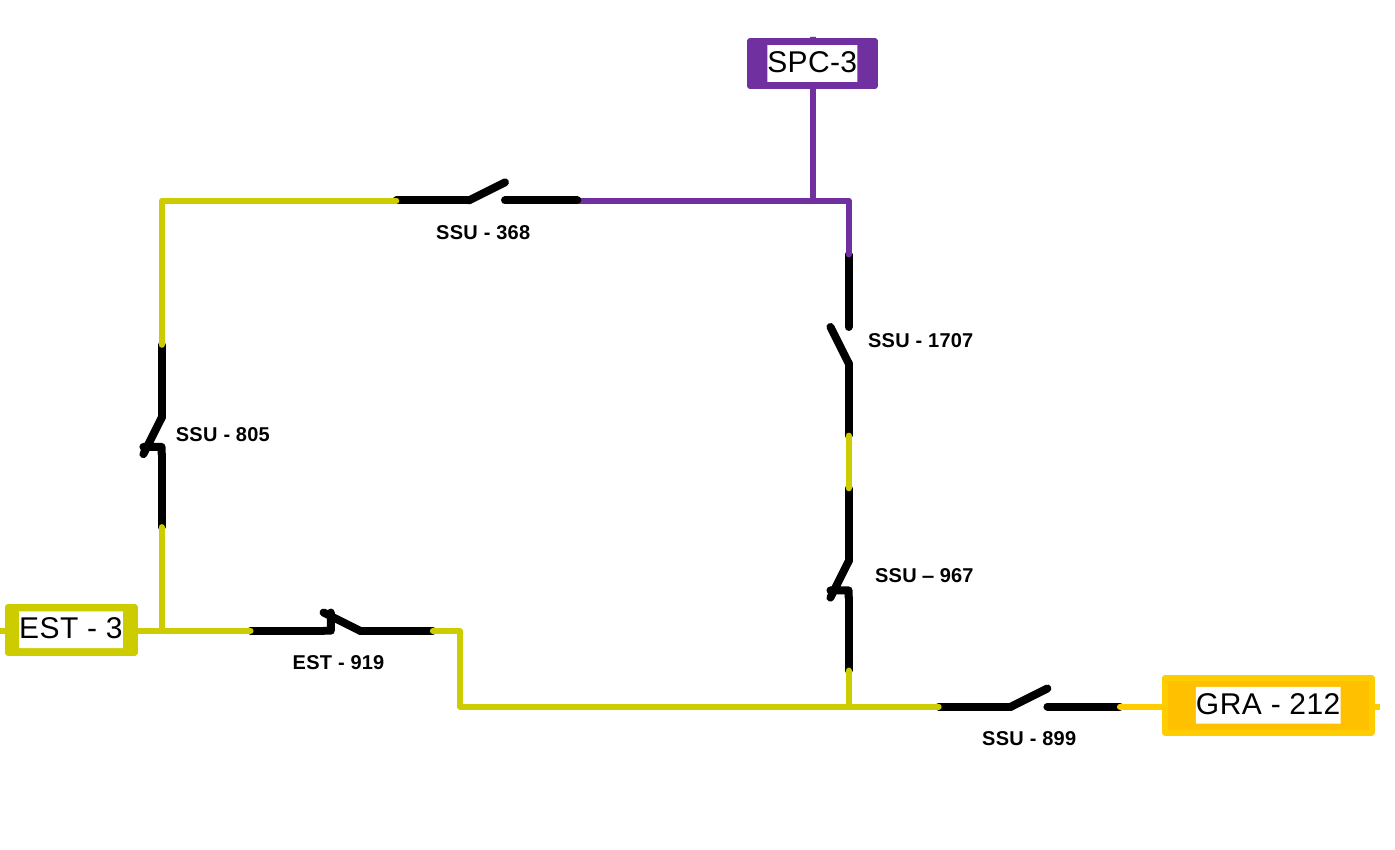
\includegraphics[width=0.7\columnwidth]{img/Caso5Unifilar}
\caption[Representa��o unifilar para os casos 6 e 7]{Representa��o unifilar dos alimentadores envolvidos no caso de teste N� 6 e 7\label{fig:Unifilar-Caso5}}
\end{figure}

 Para o defeito simulado, existem diferentes possibilidades de transfer�ncia, inclusive dividindo parte da carga para um alimentador e parte para outro, caso n�o seja poss�vel transferir toda carga para um alimentador apenas. A metodologia detectou 3 poss�veis transfer�ncias v�lidas que est�o apresentadas na Tabela \ref{caso5-Resultados}. As manobras 2 e 3 n�o podem ser aplicadas simultaneamente, uma vez que elas colocariam os alimentadores ``GRA - 212'' e ``SPC - 3'' em um ciclo, o que n�o seria uma solu��o v�lida. Dessa forma somente uma das duas ser� executada, nesse caso, a que possui menor carregamento nos condutores, a manobra 2.

\begin{table}[htbp]
\caption{Resultados para o caso de estudo 6}
\begin{tabular}{|c|c|c|r|r|r|r|}
\hline
\multicolumn{1}{|c|}{Manobra} & Abrir & Fechar & \multicolumn{1}{c|}{Clientes} & \multicolumn{1}{c|}{Condutores (\%)} & \multicolumn{1}{c|}{Prote��o (\%)} & \multicolumn{1}{c|}{Queda (\%)} \\ \hline
1\textdegree &  SSU - 805  &  SSU - 368  & 2663 & 33,8778 & 19,3103 & 0,3302 \\ \hline
2\textdegree & EST - 919 & SSU - 899 & 4806 & 47,0291 & 58,7864 & 2,4695 \\ \hline
3 & EST - 919 & SSU - 1707 & 4806 & 51,2545 & 31,1837 & 0,7775 \\ \hline
\end{tabular}
\label{caso5-Resultados}
\end{table}


\subsection[Caso 7] {Caso 7: Transfer�ncia para diferentes alimentadores, com divis�o de carga}
Para testar o caso de dividir a carga em diferentes alimentadores, foi feita uma simula��o em hor�rio diferente dos demais (6:00) e com o seguinte ajuste de carga:
\begin{description}
 \item [EST - 3:] 130 A;
 \item [SPC - 3:] 80 A;
 \item [GRA - 212:] 140 A.
\end{description}

Em compara��o com as manobras anteriores, apresentadas na Tabela \ref{caso5-Resultados}, se as mesmas fossem aplicadas nessa condi��o do sistema de distribui��o, os resultados possuiriam restri��es e poderiam transferir apenas 2663 consumidores. Os valores de tais manobras est�o na Tabela \ref{tab:caso5-Manobras-invalidas}, onde pode-se notar o violamento das restri��es das manobras 1 e 2, sendo 118\% de carregamento dos condutores e de 96\% dos equipamentos de prote��o respectivamente nas manobras. Apenas a manobra entre as chaves ``SSU - 805'' e ``SSU - 368'' pode ser aplicada.

\begin{table}[htbp]
\caption{Manobras do caso 6 aplicadas �s 6:00}
\begin{tabular}{|c|c|c|r|r|r|r|}
\hline
\multicolumn{1}{|c|}{Manobra} & Abrir & Fechar & \multicolumn{1}{c|}{Clientes} & \multicolumn{1}{c|}{Condutores (\%)} & \multicolumn{1}{c|}{Prote��o (\%)} & \multicolumn{1}{c|}{Queda (\%)} \\ \hline
1$^\dag$ &  SSU - 967  &  SSU - 1707  & 4806 & 118,340 & 67,4538 & 1,69866 \\ \hline
2$^\dag$ &  EST - 919  &  SSU - 899  & 4806 & 77,514 & 96,8924 & 3,90202 \\ \hline
3\textdegree &  SSU - 805  &  SSU - 368  & 2663 & 102,482 & 58,4148 & 1,01778 \\ \hline
\end{tabular}
\label{tab:caso5-Manobras-invalidas}
\end{table}

A metodologia foi capaz de contornar essas viola��es com o uso de transfer�ncias que dividem a carga entre diferentes alimentadores e, com isso, conseguiu transferir todos os consumidores que se encontram ap�s o defeito sem violar nenhuma das restri��es. Tais manobras s�o apresentadas na Tabela \ref{caso5-Resultados-600}.

\begin{table}[htbp]
\caption{Resultados para o caso de estudo 7. Simulado �s 6:00}
\begin{tabular}{|c|c|c|r|r|r|r|}
\hline
\multicolumn{1}{|c|}{Manobra} & Abrir & Fechar & \multicolumn{1}{c|}{Clientes} & \multicolumn{1}{c|}{Condutores (\%)} & \multicolumn{1}{c|}{Prote��o (\%)} & \multicolumn{1}{c|}{Queda (\%)} \\ \hline
1\textdegree &  SSU - 967  &  SSU - 1707  & 2083 & 91,5521 & 52,1847 & 0,90991 \\ \hline
2\textdegree &  EST - 919  &  SSU - 899  & 2723 & 67,9839 & 84,9799 & 3,33808 \\ \hline
3\textdegree &  SSU - 805  &  SSU - 368  & 2663 & 102,482 & 58,4148 & 1,01778 \\ \hline
\end{tabular}
\label{caso5-Resultados-600}
\end{table}

Todas as manobras apresentadas agora podem ser executadas, mas existe uma depend�ncia entre elas, especificamente entre as manobras 1 e 2. A manobra 1 transfere parte da carga para outro alimentador e a n�mero 2 transfere o restante para outro alimentador, se essa ordem for invertida a manobra 2 iria transferir toda carga, como apresentado da Tabela \ref{tab:caso5-Manobras-invalidas}, provocando uma viola��o na restri��o dos equipamentos de prote��o.

% % Conclus�o - Obrg
\chapter{Considera��es Finais}
Este trabalho trouxe uma apresenta��o da metodologia usada para o restabelecimento autom�tico de energia el�trica considerando o uso de equipamentos telecomandados. Apesar de n�o constar nesse relat�rio, j� existe um sistema computacional que implementa a metodologia apresentada aqui e os resultados est�o satisfat�rios e dentro do esperado.

O desenvolvimento dessa metodologia para restabelecimento autom�tico, traz vantagens em rela��o a outras metodologias \cite{Gris2010} por ser aplic�vel em diferentes topologias de rede sem a necessidade de configura��o das manobras que podem ser executadas. Isso se d� pela forma que essa metodologia utiliza as informa��es em campo (medi��es, controle) com intelig�ncia computacional (simula��es, defini��es das manobras) para obter o conjunto de manobras a serem executadas para restabelecimento m�ximo do fornecimento de energia el�trica para os consumidores.

\section{Atividades Futuras}
Ficam registradas aqui as atividades para a pr�xima etapa:
\begin{itemize}
    \item Jan-Fev/12 - Complementa��o da revis�o bibliogr�fica
    \item Jan-Mar/12 - Cria��o de um cap�tulo sobre Sistemas computacionais inteligentes, onde ser�o abordadas heur�sticas e sistemas computacionais que serviram de base para o desenvolvimento desse trabalho
    \item Fev-Abr/12 - Desenvolvimento de um cap�tulo sobre redes de distribui��o, falando um pouco mais sobre automa��o e redes inteligentes
    \item Mar-Mai/12 - Expans�o da metodologia com mais exemplos e melhor apresenta��o usando alguns algoritmos.
    \item Mar-Jun/12 - Adi��o de um capitulo sobre o sistema j� desenvolvido contendo resultados para algumas redes de teste (redes reais) e alguns casos de teste usados para validar a metodologia
    \item Mai-Jun/12 - Adi��o dos anexos referentes ao desenvolvimento do sistema computacional
    \item Jun-Jul/12 - Conclus�o Disserta��o
\end{itemize}



 %Inclui arquivo conclusao.tex

% ELEMENTOS P�S-TEXTUAIS
% Refer�ncias - Obrg
\bibliography{bibliography} %Seu arquivo Bibitex

% Gloss�rio
% Ap�ndice(s)

% Anexo(s)
% \appendix

\part*{Anexos}


\chapter*{Anexo A: Dados de Carga para Previs�o}\label{anx:DadosCarga}
\renewcommand{\thefigure}{A.\arabic{figure}}

% \begin{figure}[ht]
%  \centering
%  \includegraphics[bb=0 0 794 742,scale=0.4]{../TCC-I/imagens/Instance.png}
%  % Instance.png: 915x855 pixel, 83dpi, 28.00x26.16 cm, bb=0 0 794 742
% \caption{Classes que representam uma Inst�ncia e as solu��es }
% \end{figure}
%

\begin{table}[htbp]
\centering
\caption{Dados de Carga para Previs�o de Carga}
\begin{tabular}{|r|r|r|l|}
\hline
\multicolumn{1}{|c|}{Horas} & \multicolumn{1}{c|}{Semana Anterior} & \multicolumn{1}{c|}{Carga Atual} & \multicolumn{1}{c|}{Previs�o} \\ \hline
00:00 & 72 & 79 &  \\ \hline
01:00 & 61 & 65 &  \\ \hline
02:00 & 63 & 59 &  \\ \hline
03:00 & 60 & 58 &  \\ \hline
04:00 & 55 & 57 &  \\ \hline
05:00 & 57 & 57 & \multicolumn{1}{r|}{120} \\ \hline
06:00 & 70 & 75 & \multicolumn{1}{r|}{120} \\ \hline
07:00 & 99 & 106 & \multicolumn{1}{r|}{120} \\ \hline
08:00 & 120 & 133 & \multicolumn{1}{r|}{120} \\ \hline
09:00 & 125 & 126 &  \\ \hline
10:00 & 127 & 133 &  \\ \hline
11:00 & 133 & 137 &  \\ \hline
12:00 & 92 & 95 & \multicolumn{1}{r|}{135,2717391304} \\ \hline
13:00 & 108 & 108 & \multicolumn{1}{r|}{135,2717391304} \\ \hline
14:00 & 129 & 130 & \multicolumn{1}{r|}{135,2717391304} \\ \hline
15:00 & 131 & 130 & \multicolumn{1}{r|}{135,2717391304} \\ \hline
16:00 & 129 & 131 &  \\ \hline
17:00 & 130 & 134 &  \\ \hline
18:00 & 134 & 135 &  \\ \hline
19:00 & 139 & 146 &  \\ \hline
20:00 & 125 & 142 & \multicolumn{1}{r|}{142} \\ \hline
21:00 & 115 & 132 & \multicolumn{1}{r|}{142} \\ \hline
22:00 & 105 & 118 & \multicolumn{1}{r|}{142} \\ \hline
23:00 & 92 & 98 & \multicolumn{1}{r|}{142} \\ \hline
\end{tabular}
\label{}
\end{table}


\chapter*{Anexo B: Implementa��o para o Rocs}\label{anx:ProgramaRocs}
\lstinputlisting[language=C]{RocsFiles/selectManeuvers.js}

\chapter*{Anexo C: Fun��es Auxiliares para a Implementa��o}\label{anx:ProgramaRocsHelper}
\lstinputlisting[language=C]{RocsFiles/selectManeuversHelper.js}

\chapter*{Anexo D: Arquivo de Entrada do Rocs}\label{anx:EntradaRocs}
\lstinputlisting{RocsFiles/exampleGraf.graph}




\end{document}



